\documentclass{article}


\usepackage{natbib}
\usepackage{fancyvrb}
\usepackage{color}
\usepackage{graphicx}


\definecolor{royalblue}{rgb}{0.25,0.41,0.87}
\definecolor{firebrick}{rgb}{0.69,0.13,0.13}
\definecolor{chocolate}{rgb}{0.82,0.41,0.11}



\usepackage{hyperref}
\hypersetup{
pdfauthor={S. D. J. Brown},
pdftitle={Spider: Species Identity and Evolution in R. A tutorial},
bookmarks=true,
colorlinks=true,
linkcolor=chocolate,
citecolor=firebrick,
urlcolor=royalblue,
}

%################################test
%   New commands and environments
%################################

\newcommand{\spider}{\textsc{spider}} %With space at end
\newcommand{\Spider}{\textsc{Spider}} %Without space at end. Note the capital letter!
\newcommand{\scinm}{\emph}
\newcommand{\progname}[1]{\textsc{#1}}
\newcommand{\fun}[1]{\texttt{#1}}

\newcommand{\ChangeLine}[1]{%
\ifodd\value{FancyVerbLine}%
\textcolor{blue}{#1}\else\textcolor{red}{#1}\fi}


\DefineVerbatimEnvironment{console}{Verbatim}{formatcom=\color{blue}}
\DefineVerbatimEnvironment{Routput}{Verbatim}{formatcom=\color{red}}
\DefineVerbatimEnvironment{Rio}{Verbatim}{formatcom=\renewcommand{\FancyVerbFormatLine}{\ChangeLine}}{}

% \renewcommand{\FancyVerbFormatLine}[1]{%
% \ifodd\value{FancyVerbLine}%
% \textcolor{blue}{#1}\else\textcolor{red}{#1}\fi}


%################################
%   Set up text 
%################################

\setlength{\parindent}{0pt}
\setlength{\parskip}{5pt}

%################################
%   Title
%################################

\title{\Spider: Species Identity and Evolution in R.\\ A Tutorial}

\author{Samuel D.\ J.\ Brown\\\href{mailto:s_d_j_brown@hotmail.com}
{s\_d\_j\_brown@hotmail.com}\\Rupert A.\ Collins\\\href{mailto:rupertcollins@gmail.com}{rupertcollins@gmail.com}}

%################################
%   Begin the document
%################################

\begin{document}

\bibliographystyle{apa-good.bst}

\maketitle

%####################################
%####################################
%####################################

\section{Introduction}
\Spider: Species Identity and Evolution in R, is an \progname{R} package implementing a number of the most useful analyses for DNA barcoding studies and other research into species delimitation and speciation. It has been developed primarily by staff and students in the Department of Ecology at Lincoln University, and was first released in 2011. The package seeks to provide a number of analyses that the developers have found useful in their own research and hadn't been implemented in other \progname{R} packages. 

This document is a tutorial on the use of some of the functions implemented in \spider, and offers a guide to the interpretation of its output. It is intended to be useful for the beginner, so users who are familiar with \progname{R} and \progname{Ape} are encouraged to skip the first few sections. This tutorial does not discuss the basic \progname{R} syntax and data structures in detail (with a few exceptions), and the reader is referred to other manuals\footnote{The freely available \href{http://cran.r-project.org/doc/manuals/R-intro.pdf}{An Introduction to R}, \href{http://cran.r-project.org/doc/contrib/usingR.pdf}{Using R for data analysis and graphics} and \href{http://cran.r-project.org/doc/contrib/Paradis-rdebuts_en.pdf}{R for beginners} are particularly recommended} for this information.

\subsection{Conventions}

\subsubsection{Species}
\label{speciesDef}
The term ``species'' will be used a lot in this document. The creators of the package are biologists, mostly working with DNA sequences in ecology, taxonomy and systematics, and so this term is naturally the one we feel most comfortable using. However, in the context of \spider~it is important to remember that ``species'' are just an identifying tag for our group of interest, and is not necessarily limited to biological species---it can refer to any population, group, lineage or cluster of interest. 

\subsubsection{R commands}
Commands to be typed into the \progname{R} console are typeset in \texttt{\textcolor{blue}{blue typewriter}} font, while  \progname{R}'s output is typeset in \texttt{\textcolor{red}{red typewriter}} font. Functions, objects and classes mentioned in the text are typeset in \texttt{black typewriter} font.

\subsubsection{Vectors}
Character vectors will be discussed a lot, particularly in ``Species vectors'' (Section \ref{species.vectors}), so I will briefly discuss them here. Vectors form the basic \progname{R} data structure, created in the following way:

\begin{Rio}
(x <- c(1, 4, 6, 7, 2))
[1] 1 4 6 7 2
(y <- c("A", "B", "C", "F", "G"))
[1] "A" "B" "C" "F" "G"
\end{Rio}

There are many different modes of vectors, however here we will only deal with two of them: numeric and character. The first example above is a numeric vector---funnily enough, it's made up of numbers. The second is a character vector. Numbers and letters can be mixed, but the result will be a character vector. The parts of a vector will be called ``elements'' here, such that the first element of \fun{x} is 1, while that of \fun{y} is ``A''. The 2nd is 4 and ``B'' respectively, and the 4th is 7 and ``F''.

\subsubsection{Lists}
\Spider~uses lists a lot. Lists are very useful in that they are able to store in one big object, lots of other little objects bits of different classes, modes and lengths. In addition, the \fun{lapply()} function makes it easy to do the same thing to each element within a list. To demonstrate the structure of lists:

\begin{console}
testList <- list(aa = 1:5, bb = LETTERS[1:10], cc = matrix(1:4, 2))
testList
\end{console}

\begin{Routput}
$aa
[1] 1 2 3 4 5

$bb
 [1] "A" "B" "C" "D" "E" "F" "G" "H" "I" "J"

$cc
     [,1] [,2]
[1,]    1    3
[2,]    2    4
\end{Routput}

\fun{testList} contains three quite different objects, all happily coexisting. These objects can be indexed in number of ways:

\begin{Rio}
testList$aa
[1] 1 2 3 4 5
testList[[1]]
[1] 1 2 3 4 5
testList[[2]][3:5]
[1] "C" "D" "E"
testList$cc[2,]
[1] 2 4
\end{Rio}




\subsubsection{Getting help}
\progname{R} is blessed in having a large community of users that willingly offer help free of charge through avenues such as mailing lists and Stack Overflow. HOWEVER! Before even thinking of asking a question there, try looking up the documentation that comes with the program. Simply put a question mark before the function name you have a problem with and a wealth of information will appear. 

\begin{console}
?read.dna
?sppVector
\end{console}

\progname{R} help pages have a justified reputation for being dense and overwhelming at first glance, but keep trying because most of the time (particularly for the base packages) the answer is in there. It's jolly difficult writing help pages, and our attempts at it renew our appreciation for what others have produced.

If any of \spider's help pages fail to live up to standards, please send us an email, preferably with suggestions, and we'll update it accordingly.


%####################################
%####################################
%####################################

\section{Obtaining \spider}
\Spider~is a package of the statistical programming environment \progname{R}, which is available for all computing platforms from the Comprehensive R Archive Network (CRAN, \href{http://cran.r-project.org}{http://cran.r-project.org}). A stable version of \spider~is also available on CRAN, and can be downloaded from within R while connected to the internet by entering the following command at the prompt:

\begin{console}
install.packages("spider")
\end{console}

In addition to the stable version on CRAN, a development version is available at R-Forge (\href{http://spider.r-forge.r-project.org/}{http://spider.r-forge.r-project.org/}). This version can be installed from within \progname{R} by using the command:

\begin{console}
install.packages("spider", repos="http://R-Forge.R-project.org")
\end{console}

\Spider~requires the installation of the packages \progname{Ape} \citep{SW.Para.2004.ape} and \progname{Pegas} \citep{SW.Para.2010.pegas} which provide the primary data structures for working with DNA sequences and phylogenetic trees. If these packages are not already on your system, they will automatically be installed when the commands above have been run.


%####################################
%####################################
%####################################

\section{Loading data}

\subsection{Loading spider}
Once you have installed \spider, load the package using the following command: 

\begin{console}
library(spider)
\end{console}

As well as \spider, this command will load the packages \progname{Ape}, \progname{Pegas} and the required packages for \progname{Pegas}, \progname{Adegenet} \citep{Jomb.2008} and \progname{Mass} \citep{Vena.Ripl.2002}.


\subsection{Bundled datasets}
Once the packages are loaded, you are ready to go! It's now time to get some data to play with. Included in \spider~are two datasets including sequences from (appropriately enough) two New Zealand spider genera, the wolf spider genus \scinm{Anoteropsis} and the nurseryweb spider genus \scinm{Dolomedes}. These datasets have been published as \citet{Vink.Pate.2003} and \citet{Vink.Dupe.2010}. To load up these datasets, simply type: 

\begin{console}
data(anoteropsis)
data(dolomedes)
\end{console}

More information about these datasets can be discovered by having a look at these objects: 

\begin{console}
anoteropsis
\end{console}

\begin{Routput}
33 DNA sequences in binary format stored in a matrix.

All sequences of same length: 409 

Labels: Artoria_flavimanus Artoria_separata Anoteropsis_adumbrata_CO 
Anoteropsis_adumbrata_BP Anoteropsis_aerescens_MK Anoteropsis_aerescens_TK ...

Base composition:
    a     c     g     t 
0.261 0.135 0.159 0.445
\end{Routput}

\begin{Rio}
class(anoteropsis)
[1] "DNAbin"
dolomedes
\end{Rio}

\begin{Routput}
37 DNA sequences in binary format stored in a matrix.

All sequences of same length: 850 

Labels: minorD003 minorD031 minorD026 minorD030D056 minorD006 
minorD014D017D042D043 ...

Base composition:
    a     c     g     t 
0.254 0.123 0.181 0.443
\end{Routput}

\begin{Rio}
class(dolomedes)
[1] "DNAbin"
\end{Rio}

This tells us a whole bunch of stuff. Starting from the top, the first line tells us how many sequences are in the alignment, and if these sequences are stored as a list or as a matrix. This latter piece of information is handy to know if we want to manipulate them further down the track. The next line tells us the length of the sequences, including the minimum, maximum and average if the sequences are of different lengths. The third line shows the names of the first few sequences to give us an idea of the naming scheme, and finally the base composition of the alignment is given.

\subsection{Loading your own}
While the above datasets give us something to work on for the rest of the tutorial, what is a lot more interesting is working on your own datasets. To load your own datasets into \spider, use the function \fun{read.dna()} supplied by \progname{Ape}. This function can read DNA sequence files encoded in the \href{http://cmgm.stanford.edu/phylip/formats.html#6}{\progname{Phylip}} sequential or interleaved formats, \progname{Clustal}, or (my preferred option) \progname{Fasta} format. To load sequences stored in a \progname{Fasta} formatted file called ``mySequences.fas'' in the ``R'' folder in your ``My Documents'', use the following commands:

\begin{console}
setwd("C:\\My Documents\\R")
dat <- read.dna("mySequences.fas", format="fasta")
dat
\end{console}

The first line (\fun{setwd()}) sets the working directory for the \progname{R} session. Every other file that you read or write for the duration of your session will end up in the directory specified here (unless you change it later in the session).

If all sequences in the alignment are the same length, \fun{read.dna()} stores the result as a matrix. The names of these sequences can be retrieved using the command \fun{dimnames(dat)}. This command results in a list, the first element of which contains the rownames (in this case the sequence names), the second contains the column names (in this case empty). Thus, the names of sequences can be obtained using \fun{dimnames(dat)[[1]]}.

If the alignment contains sequences of different lengths, \fun{read.dna()} stores the result as a list. When this occurs, the names of the sequences can be retrieved using \fun{names(dat)}. 

\subsection{Getting sequences from GenBank}
\href{http://www.ncbi.nlm.nih.gov/nuccore}{GenBank} is the premier global depository for DNA sequences from all organisms. It is a huge and exciting place to visit and is an extremely valuable resource for doing all sorts of research that involves DNA. 

\progname{Ape} provides a function \fun{read.GenBank()} which allows sequences to be downloaded from the system directly into a \fun{DNAbin} object. The original version did not include information such as species names or gene regions, so a modified version is included in \spider, \fun{read.GB()}. This function works on a character vector of GenBank accession numbers, and retrieves the records that correspond to those numbers. As an example, the following code downloads 63 sequences of antarctic springtails \citep{Green.etal.2011}.

\begin{console}
seq <- 732028:732089
seq <- paste("HQ", seq, sep="")
collembola <- read.GB(seq)
\end{console}

GenBank considers the DNA sequences it stores as individuals, so the data downloaded from it are not necessarily aligned. To check properly, it is necessary to export the sequences to an external alignment editor such as \href{http://www.megasoftware.net}{\progname{Mega}} \citep{SW.Tamu.etal.2011.MEGA}, \href{http://www.mekentosj.com/science/4peaks}{\progname{4Peaks}} or \href{http://pbil.univ-lyon1.fr/software/seaview.html}{\progname{Seaview}} \citep{SW.Guoy.etal.2010.SeaView}. However,  \spider~provides a few tools for us to do a rough-and-ready job within \progname{R} itself. First of all, we'll see how long the sequences are:

\begin{console}
collLength <- sapply(collembola, length)
table(collLength)
\end{console}

\begin{Routput}
 614 618 619 624 630 631 640 658 
  1   1   2   1   1  10   1  45
\end{Routput}

The majority of sequences are 658 bp in length. We can then retain all the sequences of this length in the alignment:

\begin{console}
collembola <- collembola[which(collLength == 658)]
\end{console}

The function \fun{seeBarcode()} produces a plot that represents each base as a coloured vertical line corresponding to its nucleotide. We can use this to give us an idea if these sequences are correctly aligned or not.

\begin{console}
layout(matrix(1:6, ncol=1))
par(mar=c(0.5, 0, 0.5, 0))
apply(as.matrix(collembola)[sample(1:45,5),], MARGIN=1, FUN=seeBarcode)
seeBarcode(as.matrix(dolomedes)[sample(1:37, 1),1:658])
\end{console}

This code plots the sequences for 5 randomly sampled \fun{collembola} and one \fun{dolomedes}. The results can be seen in Figure \ref{seeBarcode.fig}. The top 5 all show reasonably similar patterns of variation. In particular, the blue, yellow \& red, blue pattern in the second quarter is consistent across all \fun{collembola} sequences. Compared to the \fun{dolomedes} sequence, the difference is clear. For the purpose of the rest of the document, I'll assume the sequences in \fun{collembola} are correctly aligned. As mentioned above, however, in other analyses it will be necessary to determine this with greater certainty.

\begin{figure}[tbp]
	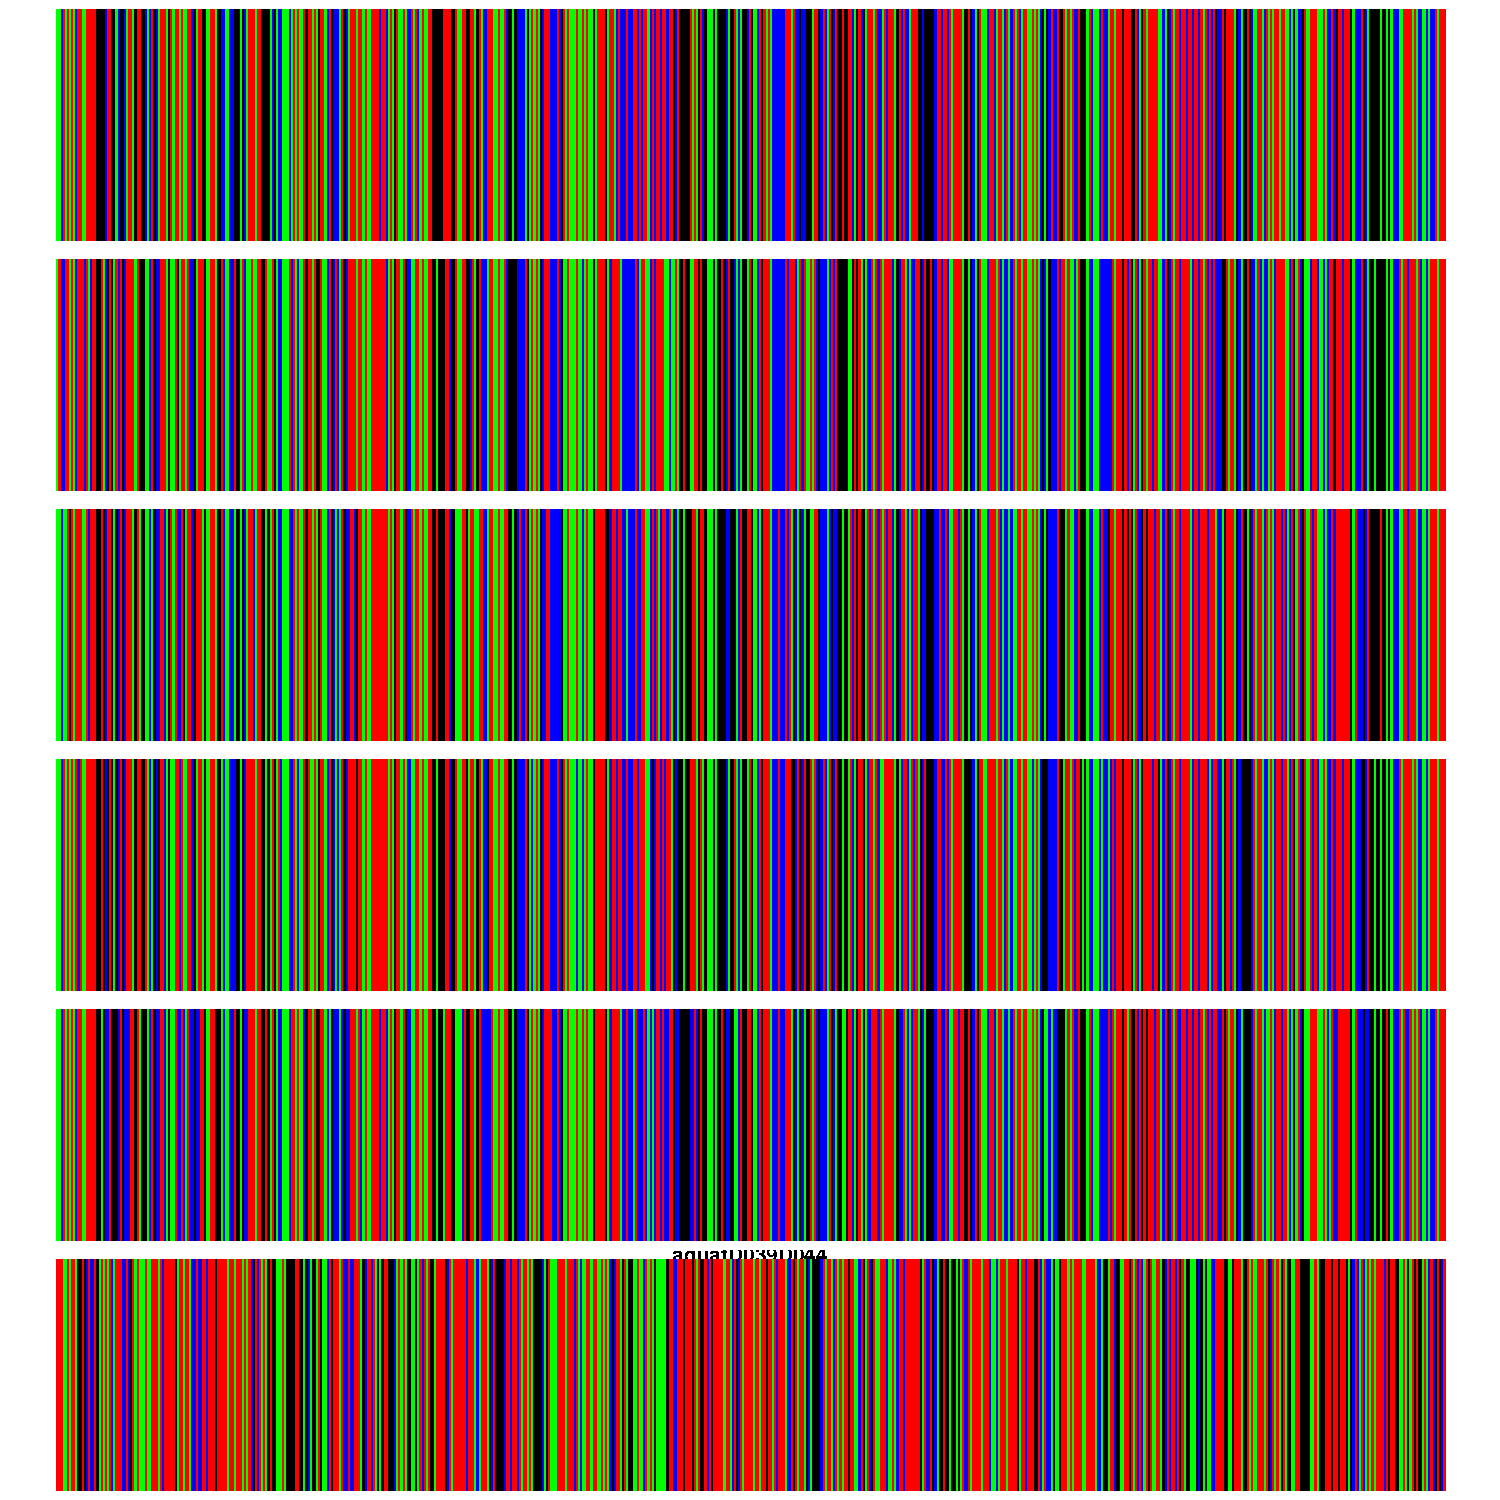
\includegraphics[width=\textwidth]{seeBarcode}
	\caption{Five random \fun{collembola} sequences and one from \fun{dolomedes} to determine if sequences are roughly in alignment}
	\label{seeBarcode.fig}
\end{figure}



\subsection{Getting sequences from BOLD}
\label{BOLD.section}
The \href{http://www.barcodinglife.com}{Barcode of Life Data System (\progname{Bold})} is the data storage portal for a global endeavour to catalogue the living world, using short (around 650 bp) DNA sequences from standard gene regions \citep{Ratnasingham2007}. The bulk of this data comes from the mitochondrial gene region cytochrome \emph{c} oxidase I (COI). There are a lot of sequences in the database, but unfortunately only a small portion of them are currently made public. \Spider~contains functions for searching and downloading sequences from \progname{Bold}. We will download some sequences of \scinm{Trigonopterus} weevils from northern New Guinea rainforest that show high levels of diversity \citep{Ried.etal.2010,Ried.2010}

\begin{console}
nums <- search.BOLD("Trigonopterus")
weevils <- read.BOLD(nums)
\end{console}

The function \fun{search.BOLD()} searches the database and retrieves the specimen numbers for the records matching the search term. These numbers are then used by \fun{read.BOLD()} to download the sequences.

NB: At the moment, the eFetch system for downloading sequences (used by \fun{read.BOLD}) returns the same records three times. I emailed the good people at \progname{Bold} about it, but it is yet to be rectified. The line below will remove these triplicate records, but hopefully the problem will be fixed in the near future.

\begin{console}
weevils <- weevils[match(unique(names(weevils)), names(weevils))]
\end{console}

If you have a look at the \fun{weevils} object, you'll see that the sequence length is given as 1,500 bp. Later on though, we'll find that most of this length is made up of missing data, so we'll cut it down to size.

\begin{console}
weevils <- as.matrix(weevils)[,1:700]
\end{console}

We now have an alignment that is only 670 bp long. Less than half of the original size. Much better!


%####################################
%####################################
%####################################

\section{Species vectors}
\label{species.vectors}

\subsection{What they're all about}
Species vectors are the method used by \spider~to distinguish between the species in the dataset. They are simply a character vector that is the same length as the number of individuals in the dataset. The elements in the species vector correspond to the individuals in the dataset, so order is very important. The elements must also be \emph{consistent within} each species, and \emph{unique between} them. In the terminology for this document, ``species vector'' refers to the whole object, while ``species index'' refers to individual elements within it. I will reiterate here, that the term ``species'' can refer to any grouping structure that you care to use. See Section \ref{speciesDef} for more details on how ``species'' is used in this document.

Examples of species vectors and different methods of creating them are discussed below. 

% \subsection{A basic species vector}

% The following block of code creates a randomly generated tree and plots the tiplabels showing the species vector we created for this tree.

% \begin{console}
% set.seed(13)
% tr <- rtree(9)
% speciesVector <- c("A", "A", "B", "B", "C", "C", "D", "D", "D")
% plot(tr)
% tiplabels(speciesVector, adj=c(-2,0.5))
% \end{console}

\subsection{Extracting the species vector from pre-named labels}
Most of the biologists I've come across name their sequences with a  system that incorporates the species identity into it in some way, shape or form. The \fun{anoteropsis} and \fun{dolomedes} datasets demonstrate two different methods of incorporating the information into the labels.

\subsubsection{\fun{anoteropsis} species vector}

\begin{console}
head(dimnames(anoteropsis)[[1]])
\end{console}

\begin{Routput}
[1] "Artoria_flavimanus"       "Artoria_separata"        
[3] "Anoteropsis_adumbrata_CO" "Anoteropsis_adumbrata_BP"
[5] "Anoteropsis_aerescens_MK" "Anoteropsis_aerescens_TK"
\end{Routput}

In \fun{anoteropsis} the labels are made up of the genus and species separated by an underscore. When more than one specimen per species is included, the geographic locality is also included, separated again by an underscore. The species vector can easily be constructed by splitting apart each element at the underscore (using \fun{strsplit()}), and pasting the first two parts together again (using a combination of \fun{paste()} and \fun{sapply()}). To put it all together:

\begin{console}
aa <- strsplit(dimnames(anoteropsis)[[1]], split="_")
anoSpp <- sapply(aa, function(x) paste(x[1], x[2], sep="_"))
head(anoSpp)
\end{console}

\begin{Routput}
[1] "Artoria_flavimanus"    "Artoria_separata"      "Anoteropsis_adumbrata"
[4] "Anoteropsis_adumbrata" "Anoteropsis_aerescens" "Anoteropsis_aerescens"
\end{Routput}

\subsubsection{\fun{dolomedes} species vector}

\begin{console}
dimnames(dolomedes)[[1]]
\end{console}

\begin{Routput}
[28] "aquatD054"             "dondaD012D013D035"     "dondaD034"            
[31] "dondaD011"             "dondaD032D050"         "dondaD037"            
[34] "dondaD052"             "dondaD053"             "schauD007"
\end{Routput}

The labels given to \fun{dolomedes} are slightly different. The species names are abbreviated at the beginning of the label, followed by the specimen numbers possessing that haplotype. We can see though, that each species name is a set length---5 characters long. This allows us to use \fun{substr()} to extract this information:

\begin{console}
doloSpp <- substr(dimnames(dolomedes)[[1]], 1, 5)
doloSpp
\end{console}

\begin{Routput}
 [1] "minor" "minor" "minor" "minor" "minor" "minor" "minor" "minor" "minor"
[10] "minor" "minor" "minor" "minor" "minor" "minor" "minor" "aquat" "aquat"
[19] "aquat" "aquat" "aquat" "aquat" "aquat" "aquat" "aquat" "aquat" "aquat"
[28] "aquat" "donda" "donda" "donda" "donda" "donda" "donda" "donda" "schau"
[37] "schau"
\end{Routput}


\subsubsection{\fun{collembola} species vector}
\begin{console}
names(collembola)
\end{console}

\begin{Routput}
 [1] "HQ732028 | Anurida_maritima"                    
 [2] "HQ732029 | Ceratophysella_cf._gibbosa_CADH-2011"
 [3] "HQ732030 | Ceratophysella_denticulata"          
 [4] "HQ732031 | Ceratophysella_denticulata"          
 [5] "HQ732032 | Ceratophysella_denticulata" 
\end{Routput}

The species vector for the \fun{collembola} sequences we downloaded from GenBank can be retrieved in two ways. First, the harder way, which involves splitting the \fun{names()} of the alignment at the pipe:

\begin{console}
collSpp <- strsplit(names(collembola), split=" \\| ")
collSpp <- sapply(collSpp, function(x) x[2])
\end{console}

\begin{Routput}
 [1] "Anurida_maritima"                    
 [2] "Ceratophysella_cf._gibbosa_CADH-2011"
 [3] "Ceratophysella_denticulata"          
 [4] "Ceratophysella_denticulata"          
 [5] "Ceratophysella_denticulata" 
\end{Routput}

Note the double slash in front of the ``\verb+|+''. This is because the ``\verb+|+'' is a restricted character in \progname{R} and the double slash tells it that we actually mean the character, not the symbol.

The easy way is to make use of the \fun{attr()} slot that \fun{read.GB()} tacks on the end of the object:

\begin{console}
attr(collembola, "species")
\end{console}

Which results in exactly the same thing. 

\subsubsection{\fun{weevils} species vector}

\begin{console}
names(weevils)
\end{console}

\begin{Routput}
  [1] "GBCL5258-09|Trigonopterus_sp._spz"  "GBCL5259-09|Trigonopterus_sp._sph" 
  [3] "GBCL5260-09|Trigonopterus_sp._sph"  "GBCL5261-09|Trigonopterus_sp._spw" 
  [5] "GBCL5262-09|Trigonopterus_sp._spw"  "GBCL5263-09|Trigonopterus_sp._spv" 
  [7] "GBCL5264-09|Trigonopterus_sp._spv"  "GBCL5265-09|Trigonopterus_sp._spr"
\end{Routput}

To get the species vector from \fun{weevils}, we could just grab the last part of the name after splitting on the underscore:

\begin{console}
weevilSpp1 <- strsplit(names(weevils), split="_")
weevilSpp1 <- sapply(weevilSpp1, function(x) x[3])
\end{console}

\begin{Routput}
  [1] "spz"  "sph"  "sph"  "spw"  "spw"  "spv"  "spv"  "spr"  "spr"  "spz" 
 [11] "spb"  "spae" "spae" "spw"  "spw"  "spv"  "spv"  "spav" "spav" "spc"
\end{Routput}

However, to make things a bit more informative I want to include the ``Trigonopterus'' part as well, though I want to drop the ``sp.'' part. This will involve splitting on both the pipe and the underscore:

\begin{console}
weevilSpp2 <- strsplit(names(weevils), split="[\\|_]")
weevilSpp2 <- sapply(weevilSpp2, function(x) paste(x[2], x[4], sep="-"))
\end{console}

\begin{Routput}
  [1] "Trigonopterus-spz"  "Trigonopterus-sph"  "Trigonopterus-sph" 
  [4] "Trigonopterus-spw"  "Trigonopterus-spw"  "Trigonopterus-spv"
\end{Routput}

The function \fun{read.BOLD()} has an \fun{attr()} slot in the same way that \fun{read.GB()} has. However, with \progname{Bold}'s current penchant for returning three of the same thing, the command \fun{attr(weevils, "species")} returns a vector three times longer than the actual number of sequences. As species vectors need to be the same length as the number of individuals in the analysis, this is not a good thing.

\subsection{Other useful functions for extracting names}
The above examples have made extensive use of a few of the \progname{R}'s key functions for manipulating character strings. Other functions worth knowing about include the \fun{grep()} family of functions, including \fun{gsub()}. These functions have the ability to search for patterns in strings, and the latter has the ability to make changes to the strings along the way. 



%####################################
%####################################
%####################################



\section{DNA barcoding}
\Spider~and R provide an ideal platform for manipulating and analysing DNA barcode data. DNA barcoding is a method of identifying of organisms using standard gene regions---particularly COI\footnote{the mitochondrial gene cytochrome \emph{c} oxidase I}---by comparing new sequences to a database of barcodes from identified and vouchered specimens. The method was first proposed by \citet{Her.etal.2003.barcoding} and has since become a global endeavour, with ongoing efforts to gather sequences and further develop the \progname{Bold} database (section \ref{BOLD.section}). Research into the utility of DNA barcoding for identification centres on determining the amount of sequence variation within and between species, and whether accurate determinations can be made. 

Calculating how effectively the DNA barcodes are able to discriminate species is usually one of the key outputs of a DNA barcoding study. In theory, the best way to do this would be to create a barcode reference library, and then independently collect additional data to test it. However, more often reference libraries are created and tested using the same data in a simulated identification scenario. The assumption is that if more data were collected, they would have a similar success rate. Testing the data involves treating each individual as an unknown query in turn, using the fact that we already know the identity of the individual from its species vector. 


\subsection{Summary statistics}
\Spider~provides two functions for determining summary statistics from your data. The first---\fun{dataStat()}---calculates the number of species and genera in the dataset, as well as the number of individuals sampled in each species. Normally the genus vector (\fun{doloGen}) would be constructed in the same way as the species vectors (section \ref{species.vectors}), but here we already know there is only one genus so don't need to extract it from the taxon names.

The second function---\fun{seqStat()}---determines sequence number and length, and reports the amount of missing data inferred from the commonly used symbols (``-, N, ?''). Except for ``N'', This function does not report ambiguous bases (e.g.\ ``R, Y, S, M'' etc)  as missing data, although they are treated as such by most other programs as well as \progname{Ape} functions such as \fun{dist.dna()}; here, we refer the user to \fun{is.ambig()}

\begin{console}
doloGen <- rep("Dolomedes", length(doloSpp))
dataStat(doloSpp, doloGen)
\end{console}

\begin{Routput}
 Genera Species     Min     Max  Median    Mean  Thresh 
      1       4       2      16      10       9       1 
\end{Routput}

The output is fairly easy to interpret. In the \fun{dolomedes} dataset we have one genus and four species. The minimum number of individuals per species is two, while the maximum is 16. The median and mean number per species is 10 and 9 respectively. The ``\fun{thresh}'' value shows how many species have fewer individuals than the threshold (default of 5). In the \fun{dolomedes} dataset, we only have one species with less than 5 individuals representing it.

Looking at the \fun{dolomedes} dataset with \fun{seqStat()} is boring---all the sequences are the same length, and there is no missing data. Therefore, we will have a look at the \fun{weevils} dataset:

\begin{console}
seqStat(weevils)
\end{console}

\begin{Routput}
   Min    Max   Mean Median Thresh 
   479    646    635    640      1
\end{Routput}

The minimum sequence length is 479 bp, while the maximum is 646. The mean and median lengths are 635 and 640 respectively, and we have one sequence that is below the default threshold value of 500 bp.


\subsection{Distance measures of identification success}

The following metrics are all based on the pairwise distance matrix between sequences. This matrix can easily be created using the \fun{dist.dna()} function provided by \progname{Ape}. The distance matrix can be calculated using various models of DNA evolution, ranging from straight raw distances, to complex models involving a lot of parameters. The standard model of evolution used in DNA barcoding studies is the Kimura 2-parameter model (K2P), which is one of the more simple models available. Conveniently, this is the default model used by \fun{dist.dna()}. It is also important when using \fun{dist.dna()}, to change the  \fun{pairwise.deletion} option to TRUE, otherwise all sites with any missing data will be deleted from all comparisons.

\begin{console}
anoDist <- dist.dna(anoteropsis, pairwise.deletion = TRUE)
doloDist <- dist.dna(dolomedes, pairwise.deletion = TRUE)
\end{console}

\subsubsection{Nearest neighbour}
The nearest neighbour criterion \fun{nearNeighbour()} simply finds the closest individual to the target, and returns the species index for that individual. If there is more than one individual that is closest to the target, the function returns the species index of the major component of the group. The default result is a logical vector that tells you if the nearest species index is the same as the individual being tested. If it is, the result is TRUE. If not, it's FALSE. Setting the \fun{names} argument to TRUE returns the name of the nearest match instead, and thus can be used to identify unknowns (subject to having tested the procedure previously of course!). The result is tabulated to ease interpretation.

\begin{console}
table(nearNeighbour(doloDist, doloSpp))
\end{console}

\begin{Routput}
FALSE  TRUE 
    1    36 
\end{Routput}

\subsubsection{BOLD identification criteria}% we changed this no? should be more options: true, false, ambig, no id ... % I also thought we removed the upper threshold as it is only for actually making an ID
The function \fun{threshID()} mimics the ``\href{http://www.barcodinglife.com/views/idrequest.php}{species identification}'' method used by \progname{Bold}. \fun{threshID()} offers a threshold based criterion (default of 1\%), looking at all specimens within the threshold of the query. There are four possible outcomes for each identification query (i.e.\ specimen in the dataset): \fun{"correct"}---all matches within the threshold of the query are the same species; \fun{"incorrect"}---all matches within the threshold are different species to the query; \fun{"ambiguous"}---both correct and incorrect species are within the threshold; \fun{"no id"}---no matches were found to any individual within the threshold . 

\begin{console}
table(threshID(anoDist, anoSpp))
\end{console}

\begin{Routput}
  correct incorrect     no id 
       11         2        20 
\end{Routput}

\subsubsection{Meier's best match}
Meier's best close match \citep{Meier.2006} is another distance-based analysis, similar to \fun{nearNeighbour()}, but it incorporates a threshold (default value of 1\%). Like \fun{threshID()}, the same four identification categories are given (\fun{"correct, incorrect, ambiguous, no id"}), but critically, this function only operates upon the single nearest-neighbour match, rather than all matches within the threshold (as with \fun{threshID()}). The ambiguous result would apply when there are more than one equally close match of different species. 

%if there are no matches within this threshold, a result of \fun{"no id"} is given. If the nearest match is the same as the test individual, the result is \fun{"correct"}, if the nearest match is different, it is \fun{"incorrect"}. This test also gives us an extra degree of uncertainty, with a result of \fun{"ambiguous"} if there is more than one species closest to the test individual.

\begin{console}
table(bestCloseMatch(anoDist, anoSpp))
\end{console}

\begin{Routput}
  correct incorrect     no id 
       11         2        20 
\end{Routput}


\subsubsection{Threshold optimisation} %% do we need to add the "localMinima" function? comes out with same result?
While the 1\% threshold used by \progname{Bold} is often a good rule of thumb, it may not always be appropriate to every dataset, and identification success can often be increased if a better threshold given the data can be found  \citep{Meye.Paul.2005}.  The function \fun{threshOpt()} provides the basis for this analysis. The function returns the number of positive identifications, the number of false negatives and the number of false positives at a given threshold. 

\begin{console}
threshOpt(doloDist, doloSpp, thresh = 0.01)
\end{console}

\begin{Routput}
     Thresh Pos False neg False pos
[1,]   0.01  28         9         0
\end{Routput}

The threshold has a default of 0.01 (= 1\%), but can be changed as the user pleases. If the threshold is changed systematically, the optimum threshold value can be determined by minimising the false positive (no conspecific matches within threshold of query) and false negative identifications (non-conspecific species within threshold distance of query). The following code shows how to create a range of threshold values (here 0.1\% to 2\%), how to test these values, and how to plot the result (Figure \ref{sensitivity.fig}). If the data contain singleton species (i.e.\ one individual per species), it is important when running this optimisation analysis to remove these, as with \fun{threshOpt()} a singleton will be a true negative, rather than a false positive identification; see \fun{rmSingletons()} for more details.

\begin{console}
threshVal <- seq(0.001,0.02, by = 0.001)
sens <- lapply(threshVal, function(x) threshOpt(doloDist, doloSpp, thresh = x))
sensMat <- do.call(rbind, sens)
barplot(t(sensMat)[3:4,], names.arg=paste((sensMat[,1]*100), "%"))
\end{console}

\begin{figure}[p]
	\centering
	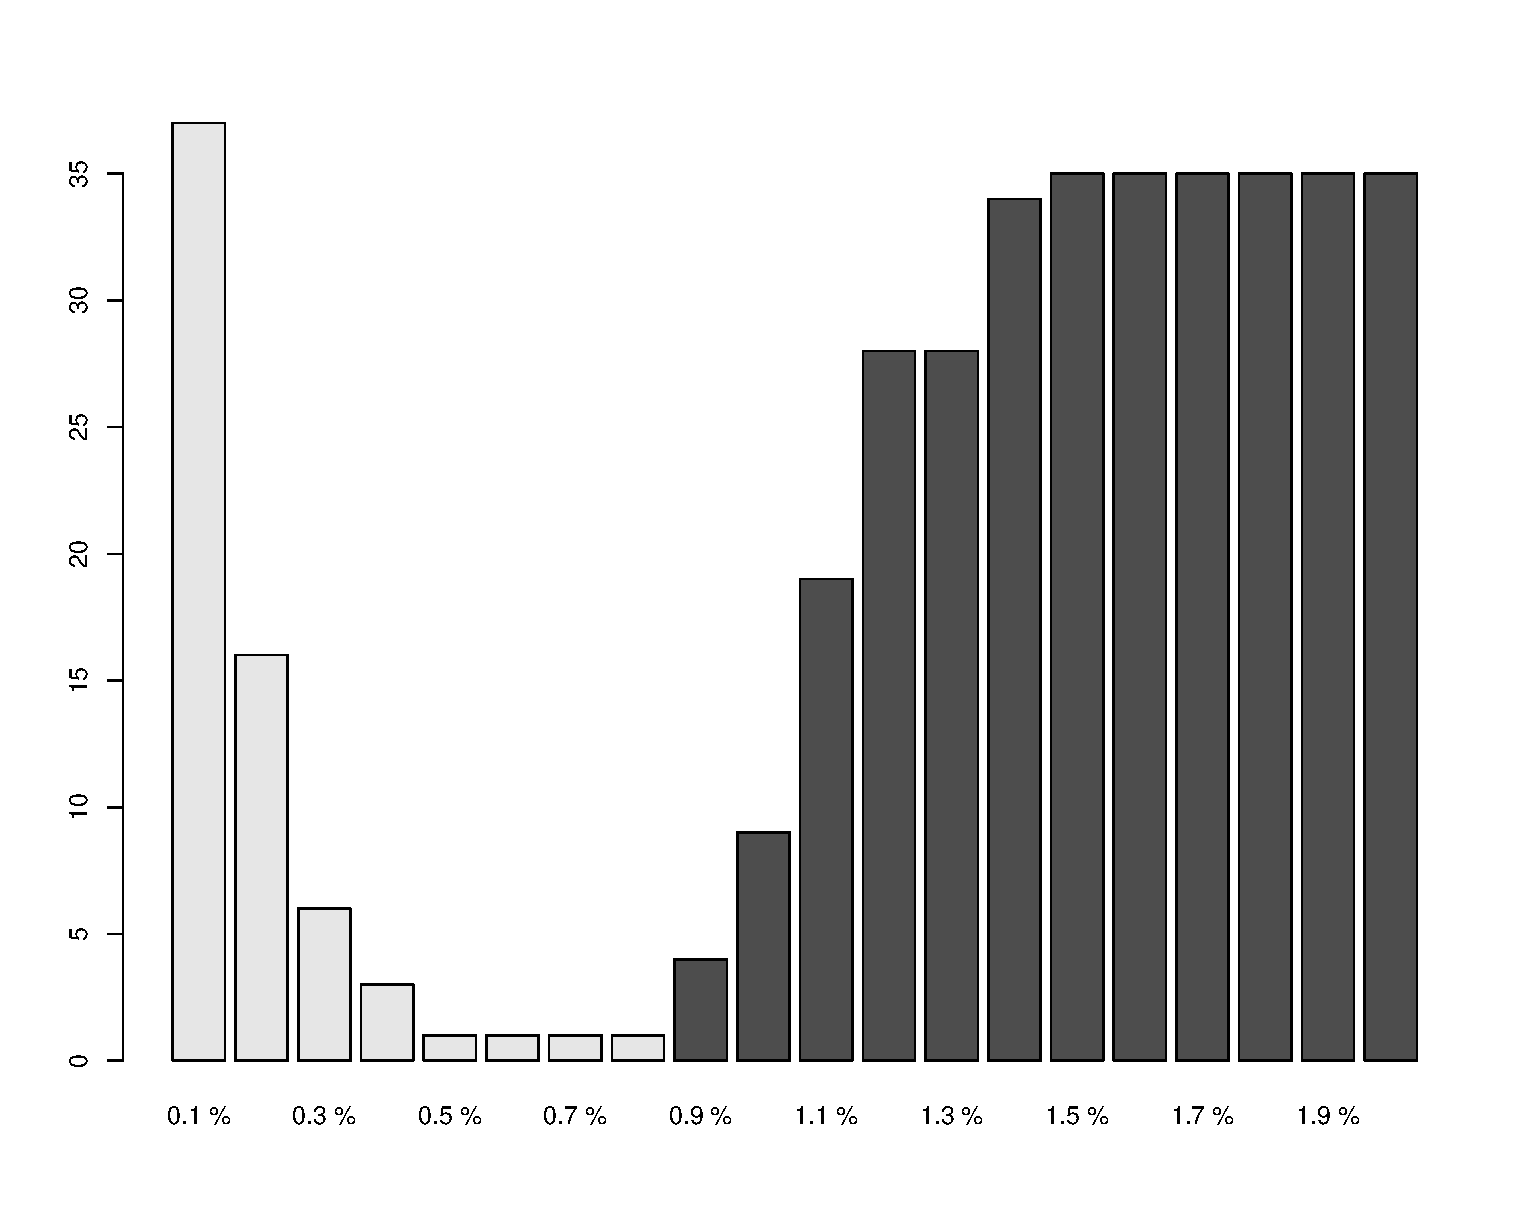
\includegraphics[width=0.9\textwidth,trim= 3cm 0cm 3cm 0cm]{sensitivity2}
	\caption{Barplot showing the false positive (light grey) and false negative (dark grey) rate of identification of \emph{Dolomedes} species as pre-set thresholds change.}
	\label{sensitivity.fig}
\end{figure}

From the figure we can see that the optimum threshold for the \fun{dolomedes} dataset is between 0.5\% and 0.8\% K2P distance. By looking at \fun{sensMat}, we confirm that these thresholds have the highest number of positive identifications at 36, and that the default 1\% is way off the mark.

\begin{Routput}
      Thresh Pos False neg False pos
 [1,]  0.001   0         0        37
 [2,]  0.002  21         0        16
 [3,]  0.003  31         0         6
 [4,]  0.004  34         0         3
 [5,]  0.005  36         0         1
 [6,]  0.006  36         0         1
 [7,]  0.007  36         0         1
 [8,]  0.008  36         0         1
 [9,]  0.009  33         4         0
[10,]  0.010  28         9         0
\end{Routput}

An experimental new function for optimising threshold values is \fun{localMinima()}. This method creates a density object from the distance matrix, and then infers where a dip in the density of genetic distances indicates the transition between intra- and inter-specific distances. A key advantage of this method, is that unlike \fun{threshOpt()}, this method does not require prior knowledge of species identity to get an indication of potential threshold values.

Here \fun{localMinima()} suggests a threshold of 0.7\%, which is entirely consistent with the results above using \fun{threshOpt()}. We would like to note, however, that \fun{localMinima()} has not yet been fully tested, but has so far yielded reliable results. We recommend further exploration of the method.

\begin{console}
doloThresh <- localMinima(doloDist)
doloThresh$localMinima[1] *100
plot(doloThresh)
\end{console}

\begin{Routput}
[1] 0.7154469
\end{Routput}


\subsubsection{The barcoding gap}

The ``barcoding gap'' \citep{Meye.Paul.2005} is an important concept in DNA barcoding. It is the assumption that the amount of genetic variation within species is smaller than the amount of variation between species. This allows the two to be distinguished. As pointed out by \citet{Meier2008}, the barcode gap should be calculated using the smallest, rather than the mean interspecific distances. \Spider~generates two statistics for each individual in the dataset, the furthest intraspecific distance among its own species---\fun{maxInDist()} and the closest, non-conspecific (i.e., interspecific distance)---\fun{nonConDist()}. Note that the distances are converted to percentages (multiply by 100).

\begin{console}
inter <- nonConDist(anoDist, anoSpp) *100
intra <- maxInDist(anoDist, anoSpp) *100
length(which(inter-intra <= 0))
\end{console}

\begin{Routput}
[1] 3
\end{Routput}

When there is no barcode gap, this is shown by a zero or negative difference when the maximum intraspecific distance (\fun{intra}) is subtracted from the minimum interspecific distance (\fun{inter}). When we use \fun{length()} and \fun{which()} to ask how many times this occurred in our dataset, we find that this was the case on three occasions.

What we may also want to do, is provide a graphical representation of the barcode gap so we can see exactly how big the differences are (Figure \ref{barcode_gap.fig}). The following code provides a very informative and pretty figure, but more importantly it gives us a tantalising glimpse into R's potential for data manipulation and plotting. 

% do we need to explain some of this code?
\begin{console}
bnd <- cbind(data.frame(inter, intra))
ord <- bnd[order(bnd$inter),]
plot(ord$inter, type="n", ylab="Percent K2P distance", xlab="Individual")
segCol <- rep("gray50", length(ord$inter))
segCol[ord$inter-ord$intra < 0] <- "red"
segments(x0=1:length(ord$inter), y0=ord$inter, y1=ord$intra, col=segCol, lwd=6)
\end{console}

\begin{figure}[p]
	\centering
	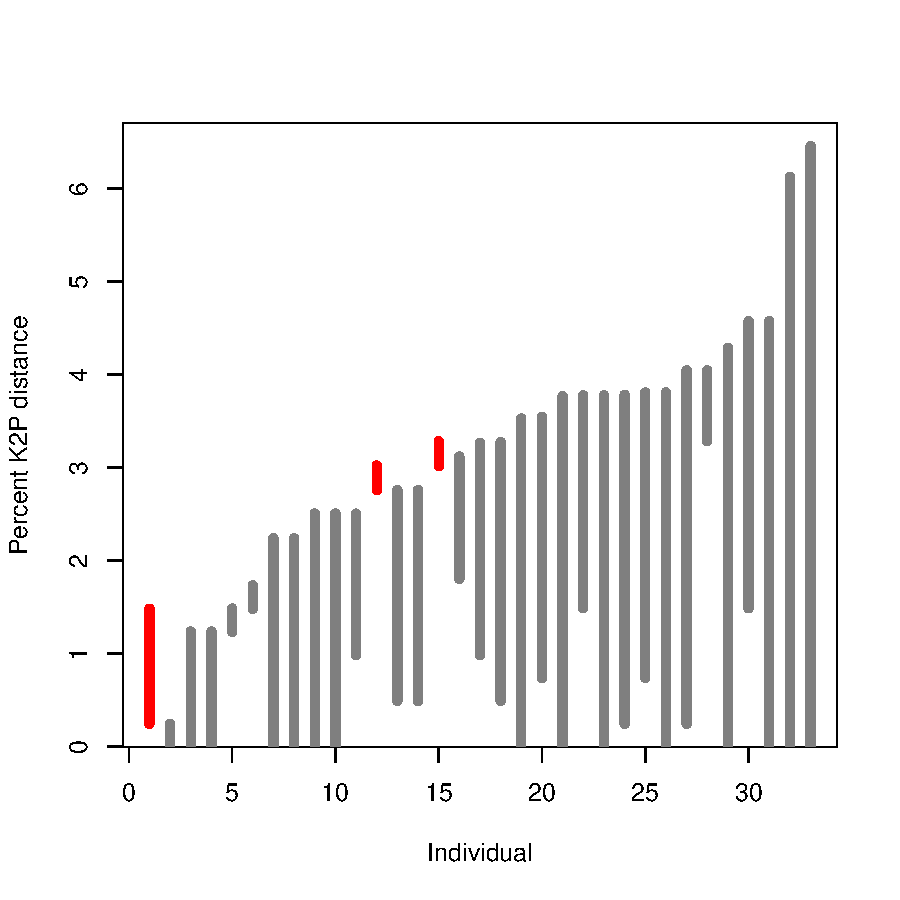
\includegraphics[width=0.7\textwidth,trim= 3cm 0cm 3cm 0cm]{barcode_gap}
	\caption{Lineplot of the barcode gap for the 33 \emph{Anoteropsis} spp. For each individual in the dataset, the grey lines represent the furthest intraspecific distance (bottom of line value), and the closest interspecific distance (top of line value). The red lines show where this relationship is reversed, and the closest non-conspecific is actually closer to the query than its nearest conspecific, i.e., the situation where there is no barcoding gap.}
	\label{barcode_gap.fig}
\end{figure}

\subsection{Tree-based measures}

\subsubsection{Species monophyly}

The species monophyly criterion determines if each species is monophyletic over a neighbour-joining (NJ) phylogram (tree). It uses a fairly simple definition of monophyly---search for clades with the same number of tips as there are species members, and see if they match. Singletons (species represented by only one individual) cause a headache. Obviously, they are either always or never monophyletic depending on your point of view. The way that \fun{monophyly()} gets around this problem is by getting the user to tell it what the point of view should be. The default is TRUE---singletons are monophyletic.

First we need to make our tree and ensure the labels are the same as the species vector. Then we can test for monophyly:

\begin{console}
anoTr <- nj(anoDist)
anoTr$tip.label <- anoSpp
monophyly(anoTr, anoSpp)
table(monophyly(anoTr, anoSpp))
\end{console}

\begin{Routput}
 [1]  TRUE  TRUE  TRUE FALSE  TRUE  TRUE  TRUE  TRUE  TRUE  TRUE  TRUE  TRUE
[13]  TRUE  TRUE  TRUE  TRUE  TRUE  TRUE  TRUE  TRUE  TRUE  TRUE

FALSE  TRUE 
    1    21
\end{Routput}

The species are ordered in the same way as \fun{unique(anoSpp)}, so this output tells us that \scinm{Anoteropsis adumbrata} is not monophyletic on this tree. However, if you've looked at the \fun{anoteropsis} dataset at all, you'll know that there are a number of singletons in this dataset. When we change the default behaviour to consider singletons as FALSE, we get a rather different picture.

\begin{console}
monophyly(anoTr, anoSpp, singletonsMono=FALSE)
table(monophyly(anoTr, anoSpp, singletonsMono=FALSE))
\end{console}

\begin{Routput}
 [1] FALSE FALSE  TRUE FALSE FALSE  TRUE FALSE FALSE FALSE FALSE FALSE FALSE
[13]  TRUE FALSE FALSE  TRUE FALSE FALSE FALSE  TRUE  TRUE FALSE

FALSE  TRUE 
   16     6 
\end{Routput}

\subsubsection{Bootstrap monophyly}

We also provide an extension to the measure of monophyly, by incorporating the bootstrap support measure. Here we use the \fun{monophylyBoot()} function with the following options: minimum of 70\% bootstrap support for a correct identification, 1000 replications, and codon based resampling for protein coding loci. 

Like many bootstrap analyses it can be lengthy to complete, and may also significantly reduce the proportion of successful identifications. We can see this from our \emph{Anoteropsis} data; there is not a single correct identification!

Because the monophyly functions work on the species, rather than individual level, the third line of code rescales the result reported in terms of the number of individuals per species---i.e., if a species is monophyletic, then all its members are also. This takes into account sampling per species, and makes the result more comparable with the individual-query distance-based methods described above.

\begin{console}
monoBoot <- monophylyBoot(anoTr, anoSpp, anoteropsis, 
singletonsMono = FALSE, reps = 1000, thresh = 0.7, block = 3)
table(monoBoot[match(anoSpp, unique(anoSpp))], useNA = "ifany")
\end{console}

\begin{Routput}
FALSE 
   33
\end{Routput}

\subsubsection{Rosenberg's probability of reciprocal monophyly}
Frequently we get excited about a specimen being different from other samples we have. Rosenberg's probability of reciprocal monophyly offers a measure to temper our excitement by bringing the sampling regime into the picture \citep{Rosenberg2007}. Rosenberg states: ``especially for small samples, an observation of monophyly for a set of lineages---even if strongly supported statistically---does not necessarily indicate that the lineages are from a distinctive group. Here I develop a test of the null hypothesis that monophyly is a chance outcome of random branching''. This is a particularly useful function for investigating support for cryptic species.

To carry out the test, a neighbour joining tree is required (\fun{anoTr}), but note that depending on the topology, sometimes the tree will have to be rooted first with \progname{Ape}'s \fun{root()} command. We then can plot colours on all the nodes that are significant to the $\alpha = 0.05$ level according to Rosenberg's random model, but this significance level can be changed \citep{Rosenberg2007}. We see in Figure \ref{rosenbergs.fig}, that very few of the nodes are red (significantly monophyletic), indicating that monophyly of some species may be due to chance, and that further sampling is required. 

\begin{console}
anoRos <- rosenberg(anoTr)
anoNodes <- anoRos < 0.05
anoLabs <- anoRos
anoLabs[anoNodes] <- "red"
anoLabs[!anoNodes] <- "grey"
plot(anoTr, cex=0.7)
nodelabels(pch=21, bg=anoLabs, node=as.numeric(names(anoLabs)), cex=2)
\end{console}

\begin{figure}[p]
	\centering
	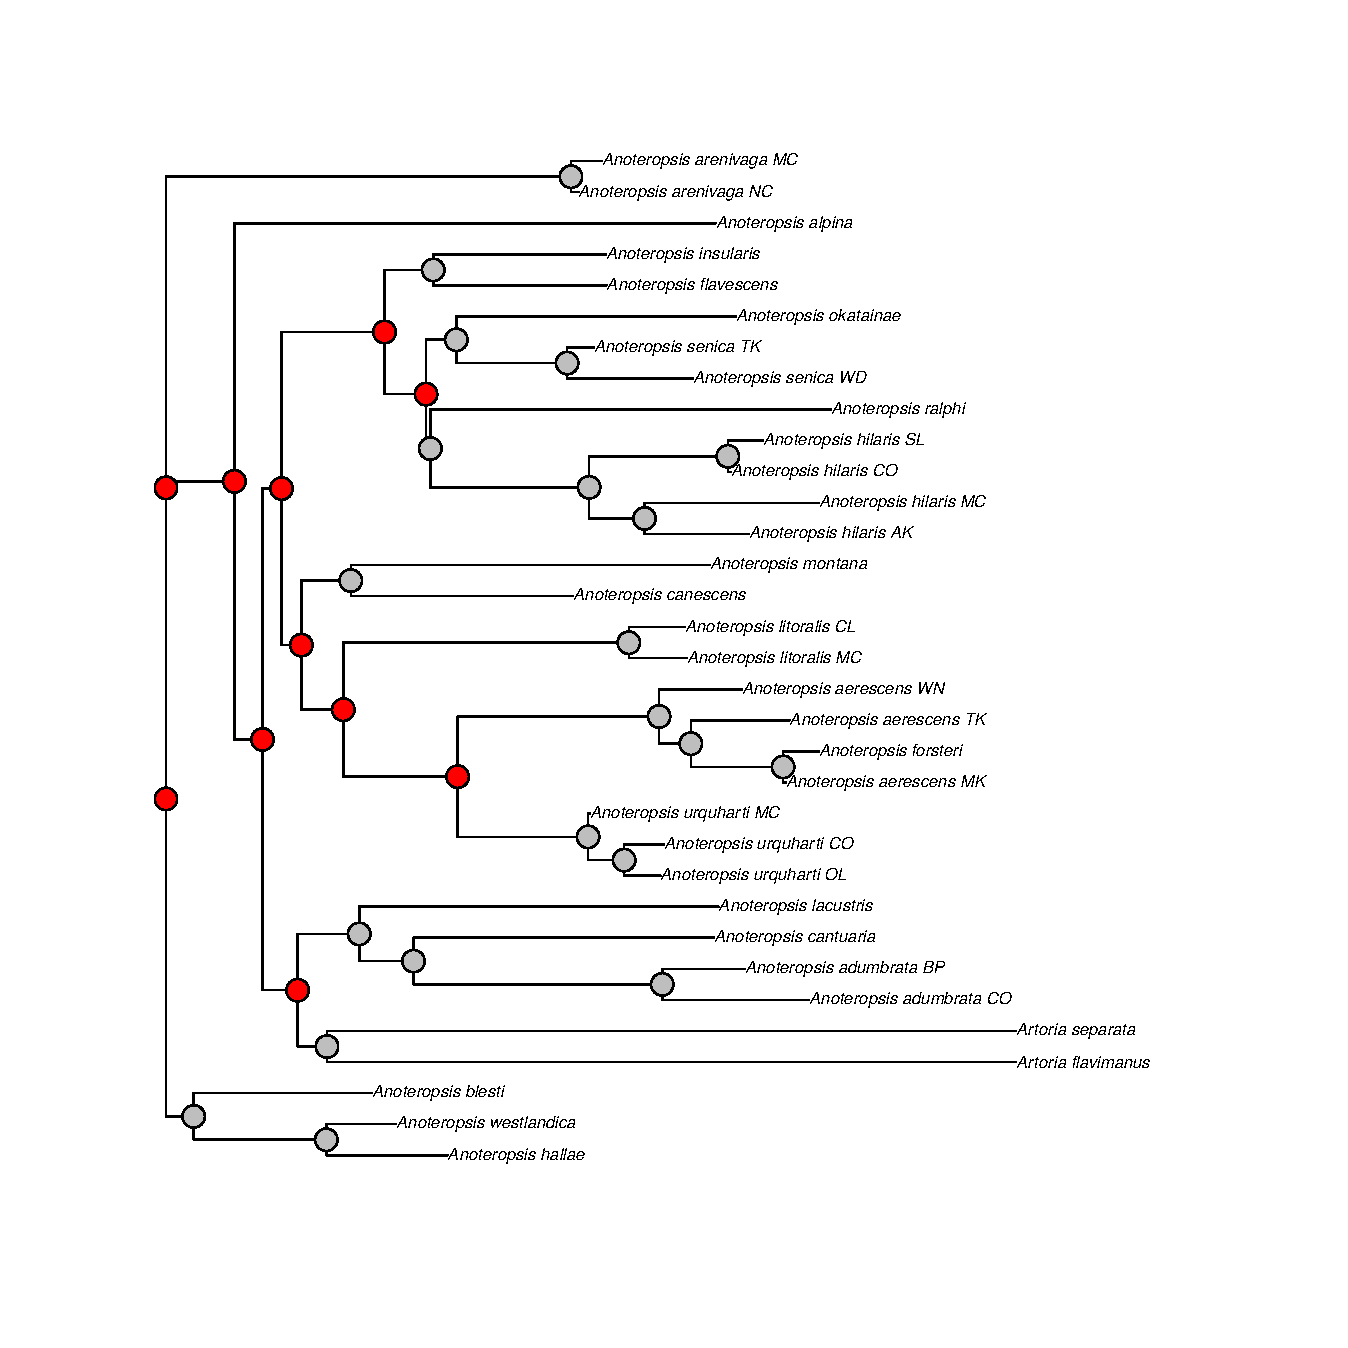
\includegraphics[width=1\textwidth, trim=3cm 1cm 3cm 0cm]{rosenbergs}
	\caption{Rosenberg's probability of reciprocal monophyly for  \emph{Anoteropsis} spp. Red nodes are significant to $\alpha = 0.05$.}
	\label{rosenbergs.fig}
\end{figure}

\subsection{Singletons}

As mentioned already, singletons (a species represented by only one individual) can be a problem for barcoding analyses \citep{Lim2011}. When treating each individual as an identification query, a singleton will not have a match available in the dataset, so will either result in an ``incorrect'' or ``no identification''---not a good result. Until databases have complete taxon coverage, singletons are likely to occur, and a real unknown specimen has a chance of not having a conspecific represented in the reference library. If your data contain a number of singleton species, it is worth additionally analysing it with the singletons removed. This will give a better identification success rate, and may be more representative of how the data may behave once fully sampled.

\Spider~can effectively deal with the singleton issue, using the \fun{rmSingletons()} function. First, we can find out how many singletons are in the data. The \fun{exclude = FALSE} option reports these singletons, and this can be compared to the number of species in the dataset.

\begin{console}
length(rmSingletons(anoSpp, exclude = FALSE))
length(unique(anoSpp))
\end{console}


\begin{Routput}
[1] 15
[1] 22
\end{Routput}


We can see that 15 of the 22 species in the dataset are singletons. Next, we can exclude these singletons and only look at species with multiple individuals. To illustrate, we will repeat the analysis of \fun{bestCloseMatch()} with both singletons included and excluded. It is important to note that the singletons are not actually removed from the analysis, they are just excluded from the results; this means the singleton individuals are still available as potential mis-matches for other species.

\begin{console}
excl <- rmSingletons(anoSpp, exclude = TRUE)
mbm <- bestCloseMatch(anoDist, anoSpp)
table(mbm[excl], useNA = "ifany")
table(bestCloseMatch(anoDist, anoSpp))
\end{console}

\begin{Routput}
  correct incorrect     no id 
       11         1         6 

  correct incorrect     no id 
       11         2        20 
\end{Routput}

We see here a huge improvement in identification success with singletons omitted (top output); there's one less ``incorrect'', and 14 fewer ``no identifications''.


%####################################
%####################################
%####################################

\section{Sliding windows} 

\subsection{The basic idea}
The principle of sliding window analysis is fairly simple---a DNA alignment is divided up into multiple smaller fragments throughout the length of the region in question. Measures of diversity \citep{Roe.Sper.2007} or questions of phylogenetic character conflict \citep{Crui.2011} can then be explored.

The \spider~function \fun{slidingWindow()} provides the base for conducting sliding window analyses. 

\begin{console}
anoWin <- slidingWindow(anoteropsis, width=50, interval=1)
length(anoWin)
\end{console}

\begin{Routput}
[1] 359
\end{Routput}

\fun{slidingWindow()} takes an alignment and slices it into pieces of \fun{width} bp each, each piece separated by \fun{interval} bp from the one before it. The result is a big list of \fun{DNAbin} objects ready and waiting to be analysed, as can be seen here:

\begin{console}
anoWin[[1]]
\end{console}

\begin{Routput}
33 DNA sequences in binary format stored in a matrix.

All sequences of same length: 50 

Labels: Artoria_flavimanus Artoria_separata Anoteropsis_adumbrata_CO 
Anoteropsis_adumbrata_BP Anoteropsis_aerescens_MK Anoteropsis_aerescens_TK ...

Base composition:
    a     c     g     t 
0.264 0.142 0.137 0.458 
\end{Routput}

\subsection{Conducting analyses}

If, for example, we wanted to see the change in GC content across the \fun{anoteropsis} sequence, we can \fun{sapply()} the \progname{Ape} command \fun{GC.content()} across our windows:

\begin{console}
anoGC <- sapply(anoWin, GC.content)
head(anoGC)
\end{console}
\begin{Routput}
[1] 0.2787879 0.2775758 0.2575758 0.2575758 0.2763636 0.2703030
\end{Routput}

If we plot the results of \fun{anoGC}, we get Figure \ref{slidWin.fig}.

\begin{figure}[tbp]
	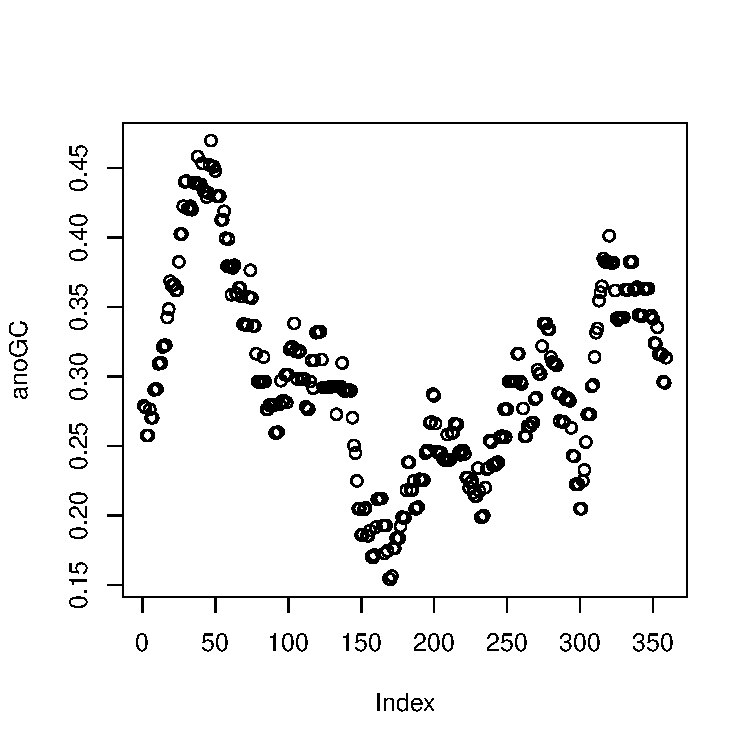
\includegraphics{slidWin}
	\caption{Average GC content of 50 bp windows across \emph{Anoteropsis} spp. sequences}
	\label{slidWin.fig}
\end{figure}

\subsection{The magic of \fun{slideAnalyses}}
A number of the most useful analyses for determining the optimum region for designing mini-barcodes \citep{Meus.etal.2008} have been implemented in the \fun{slideAnalyses()} function. This function does the whole shebang from creating the windows, to conducting the analyses. The result is a massive list detailing the data from each window. %Take note that this is our first glimpse of ``species vectors'' in action:

\begin{console}
anoAna <- slideAnalyses(anoteropsis, 50, anoSpp, interval="codons", 
distMeasures=TRUE, treeMeasures=TRUE)
\end{console}

First up: the arguments. \fun{anoteropsis} is our \fun{DNAbin} object containing our sequences, ``50'' is the desired width of the windows in question. \fun{anoSpp} is our species vector, \fun{"codons"} is a fancy way of getting an interval of 3 between our windows, \fun{distMeasures=TRUE} indicates that we want to calculate metrics based on a Kimura 2-parameter distance matrix for each window, and \fun{treeMeasures=TRUE} indicates that we want to calculate metrics based on a neighbour-joining tree monophyly from the distance matrix above. The default is that \fun{distMeasures=TRUE} and \fun{treeMeasures=FALSE} because the latter takes a lot more time to compute than the former. 

If we have a look at the object created by the function above, we get something fairly nasty:

\begin{console}
str(anoAna)
\end{console}

\begin{Routput}
List of 16
 $ win_mono_out   : num [1:120] 0.864 0.864 0.909 0.909 0.864 ...
 $ comp_depth_out : num [1:120] 0.588 0.471 0.529 0.529 0.412 ...
 $ comp_out       : num [1:120] 0.355 0.29 0.323 0.323 0.258 ...
 $ pos_tr_out     : num [1:120] 1 4 7 10 13 16 19 22 25 28 ...
 $ noncon_out     : num [1:120] 0.333 0.394 0.212 0.212 0.303 ...
 $ thres_below_out: num [1:120] 409 404 369 357 374 411 370 384 402 402 ...
 $ thres_above_out: num [1:120] 5 4 11 10 24 18 24 21 7 7 ...
 $ zero_out       : num [1:120] 0.0303 0.0398 0.0265 0.0246 0.036 ...
 $ dist_mean_out  : num [1:120] 0.0759 0.0758 0.0822 0.0848 0.0814 ...
 $ pos_out        : num [1:120] 1 4 7 10 13 16 19 22 25 28 ...
 $ dat_zero_out   : num 0
 $ boxplot_out    : logi FALSE
 $ distMeasures   : logi TRUE
 $ thresA         : num 0.2
 $ thresB         : num 0.1
 $ treeMeasures   : logi TRUE
 - attr(*, "class")= chr "slidWin"
\end{Routput}

% RUPERT: I think we need a bit more explanation of some of these?
% might need to explain what a non-conspecific distance is?
\verb|win_mono_out| is the proportion of species that are monophyletic. The closer to 1 this number gets, the more species are monophyletic.
\verb|comp_depth| and \verb|comp_depth_out| compare the clades of the trees in the window to the trees made from the full dataset. The difference is that \verb|comp_depth_out| considers only the clades that are closer to the tips of the tree than the median node depth, while \verb|comp_out| looks at all of them.
\verb|pos_out| is the position of each window (in bp) from the start of the sequence. Occasionally, trees might not be able to be made if there is too much missing data, and \verb|pos_tr_out| records the position of windows from which trees were made.
\verb|noncon_out| gives the proportion of non-conspecific distances that are 0, i.e., no difference between species. Ideally, this number would be 0 (where every species could be differentiated from one another).
\verb|thres_above_out| and \verb|thres_below_out| are the numbers of cells with distances above and below given thresholds (\verb|thresA| and \verb|thresB|). It is best if these numbers are maximised and minimised respectively.
\verb|zero_out| is the proportion of cells in the distance matrix which have a distance of 0, and can be compared with \verb|dat_zero_out| which is the same proportion in the full dataset. The closer \verb|zero_out| is to \verb|dat_zero_out|, the better.
\verb|dist_mean_out| is the mean of the distance matrix. Usually, it is best if this number is large.
Finally, the last five objects in the list are used by \fun{plot()} in creating the plots  described below.

All the information above can be presented graphically using the \fun{plot} command to produce Figure \ref{slideAnalyses.fig}:

\begin{console}
plot(anoAna)
\end{console}

\begin{figure}[tbp]
	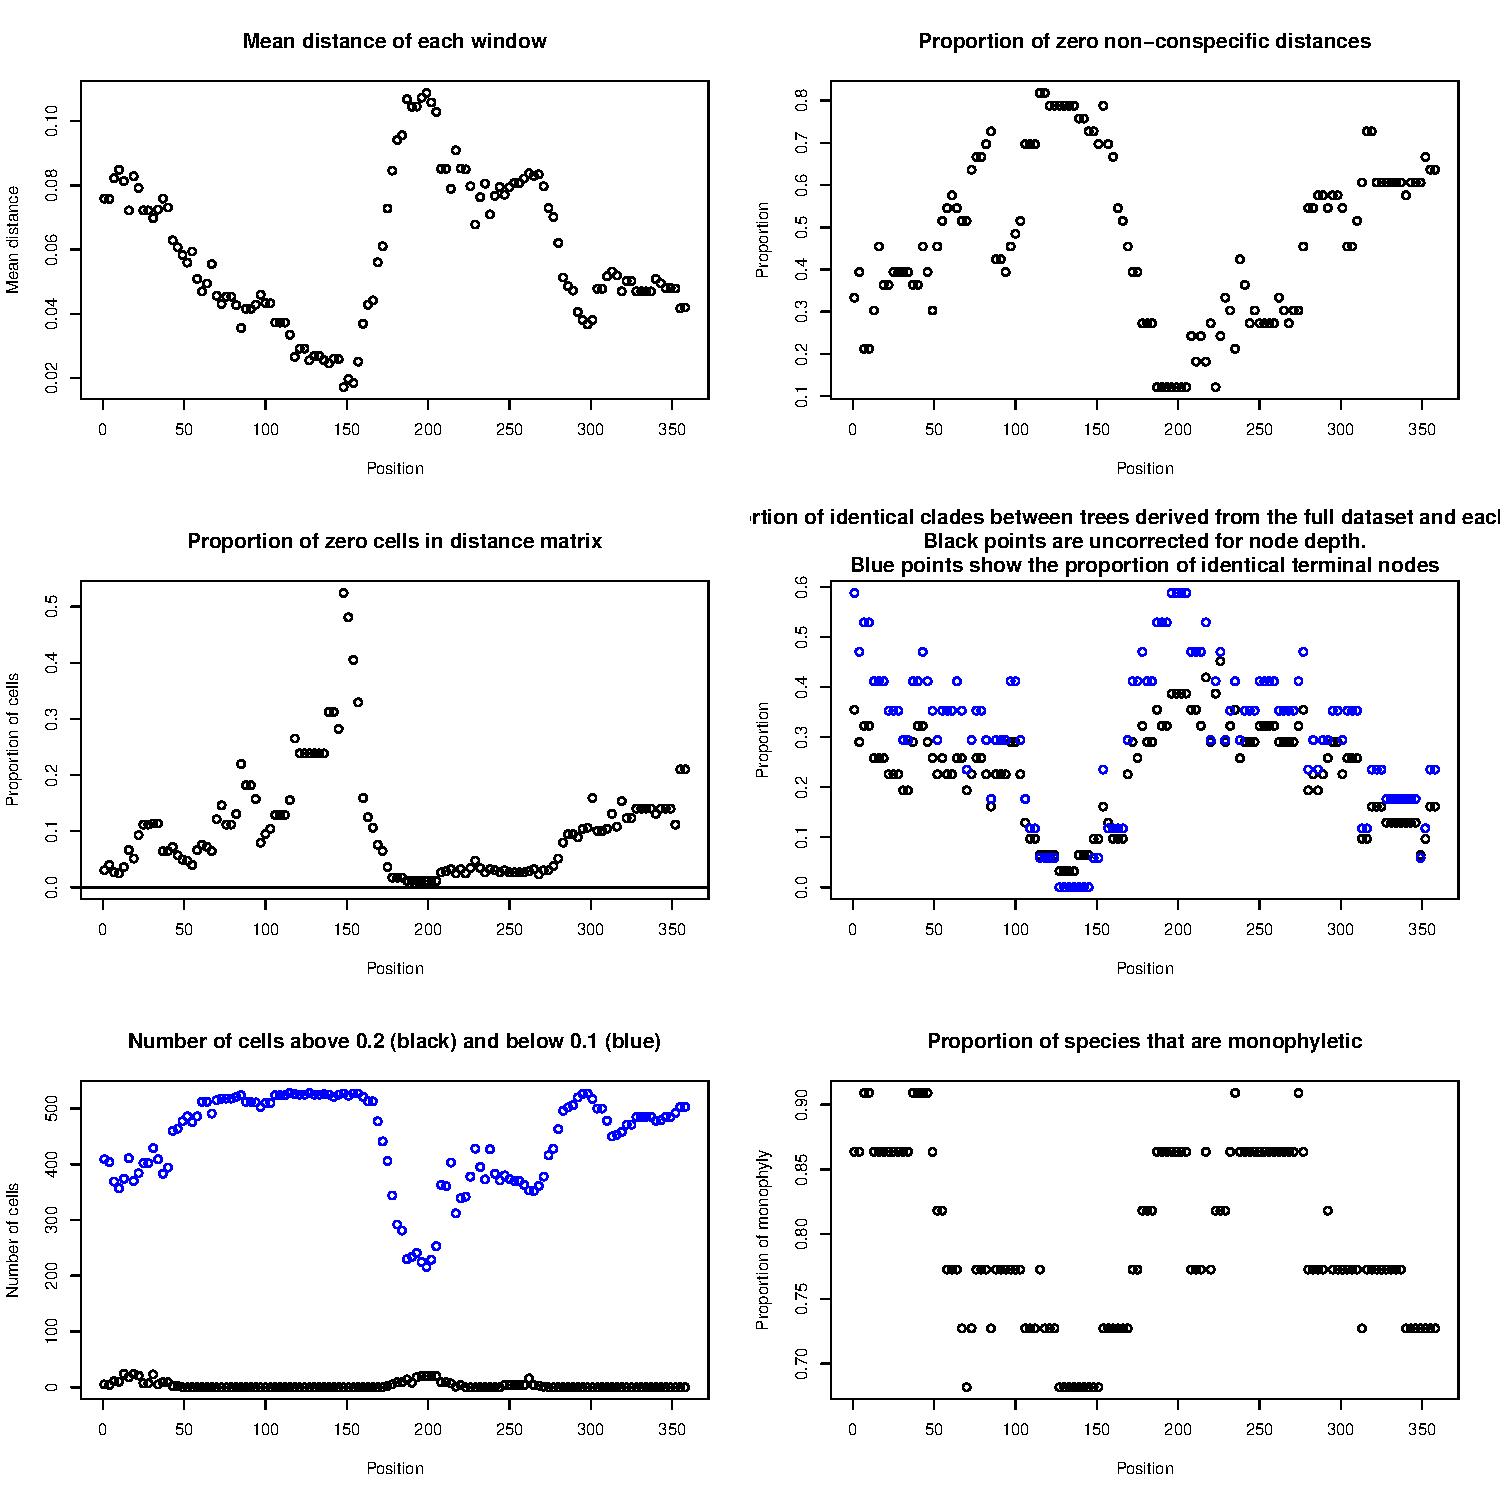
\includegraphics[width=\textwidth]{slideAnalyses}
	\caption{Results of several analyses across the COI sequences of \emph{Anoteropsis} spp. See text for more details.}%RUPERT: the "comp" figure has too much text!
	\label{slideAnalyses.fig}
\end{figure}

Starting at the top left of Figure \ref{slideAnalyses.fig}, we have the plot of the mean distance (\verb|dist_mean_out|). We see that this is at its greatest at the 200 bp position, and at its lowest around 150 bp. Next one down the column, we have the proportion of zero cells in the distance matrix (\verb|zero_out|). Once again, this is minimised around 200 bp and is at its highest at 150 bp. The unbroken horizontal line crossing the y-axis at 0 is the proportion of zero cells in the distance matrix created from the full dataset (\verb|dat_zero_out|). At the bottom of the first column, we have the number of cells above and below the thresholds (\verb|thres_above_out| and \verb|thres_below_out|). The two metrics meet their maximum and minimum respectively at (surprise, surprise!) 200 bp. The top right plot displays the proportion of zero non-conspecific distances, which find their minimum at 200 bp, but is greatest (a scary 0.8) around 100 bp. The middle right plot shows the proportion of clades that are identical between the windows and the full dataset. Black nodes comprise all clades, while the blue ones are a subset making up the shallower clades. In this example they're mixed up with each other, due to the fact that this dataset has few representatives of each species. For datasets including lots of conspecific individuals, there is greater separation between the blue and the black points. As we've come to expect though, both measures are pretty high at 200 bp and low at 140 bp. Finally, at the bottom right we have the proportion of species that are monophyletic. Unlike previous measures, it appears that the 50 bp mark is best (though 200 bp is fairly respectable), but 140 is still in the doldrums. All in all, these plots consistently indicate that the best region for creating 50 bp mini-barcodes is around the 200 bp mark.

The information can also be shown as a table that ranks the windows, showing by default the top 10 windows:

\begin{console}
rankSlidWin(anoAna)
\end{console}

\begin{Routput}
   position mean_distance monophyly clade_comparison clade_comp_shallow
67      199    0.10878089 0.8636364        0.3870968          0.5882353
66      196    0.10733553 0.8636364        0.3870968          0.5882353
68      202    0.10581874 0.8636364        0.3870968          0.5882353
69      205    0.10287159 0.8636364        0.3870968          0.5882353
63      187    0.10685304 0.8636364        0.3548387          0.5294118
65      193    0.10453572 0.8636364        0.3225806          0.5294118
64      190    0.10446778 0.8636364        0.3225806          0.5294118
4        10    0.08482881 0.9090909        0.3225806          0.5294118
3         7    0.08223324 0.9090909        0.3225806          0.5294118
73      217    0.09090806 0.8636364        0.4193548          0.5294118
   zero_noncon zero_distances above_threshold below_threshold
67   0.1212121     0.01136364              20             216
66   0.1212121     0.01136364              20             225
68   0.1212121     0.01136364              20             229
69   0.1212121     0.01136364              20             253
63   0.1212121     0.01136364              14             230
65   0.1212121     0.01136364              18             241
64   0.1212121     0.01136364               8             234
4    0.2121212     0.02462121              10             357
3    0.2121212     0.02651515              11             369
73   0.1818182     0.02462121               1             312
\end{Routput}

It shows the same conclusion that we drew from the graphical representation of the data, namely that the windows around the 200 bp mark are particularly good by most of the criteria. The default behaviour of \fun{rankSlidWin()} is that it returns the best summed over all critera, but other criteria can be used to rank the windows. See the help page of \fun{rankSlidWin()} for more details.

\subsection{Plots of boxes}
Another way of looking at the variation across the sequences is by plotting boxplots that show the distribution of pairwise genetic distances of each window. This can be done by using the function \fun{slideBoxplots()}. This function has three methods that be used. \fun{"overall"} shows a single boxplot that represents the whole distance matrix, \fun{"interAll"} separates the distances into intra- and inter-specific distances and plots a boxplot of each. This differs from \fun{"nonCon"} (the default) in that \fun{"nonCon"} restricts the inter-specific distances to only the nearest non-conspecific distance for each individual in the dataset.

\begin{console}
anoBox <- slideBoxplots(anoteropsis, 50, anoSpp, interval="codons", 
method="nonCon")
plot(anoBox)
\end{console}

\begin{figure}[p]
	\centering
	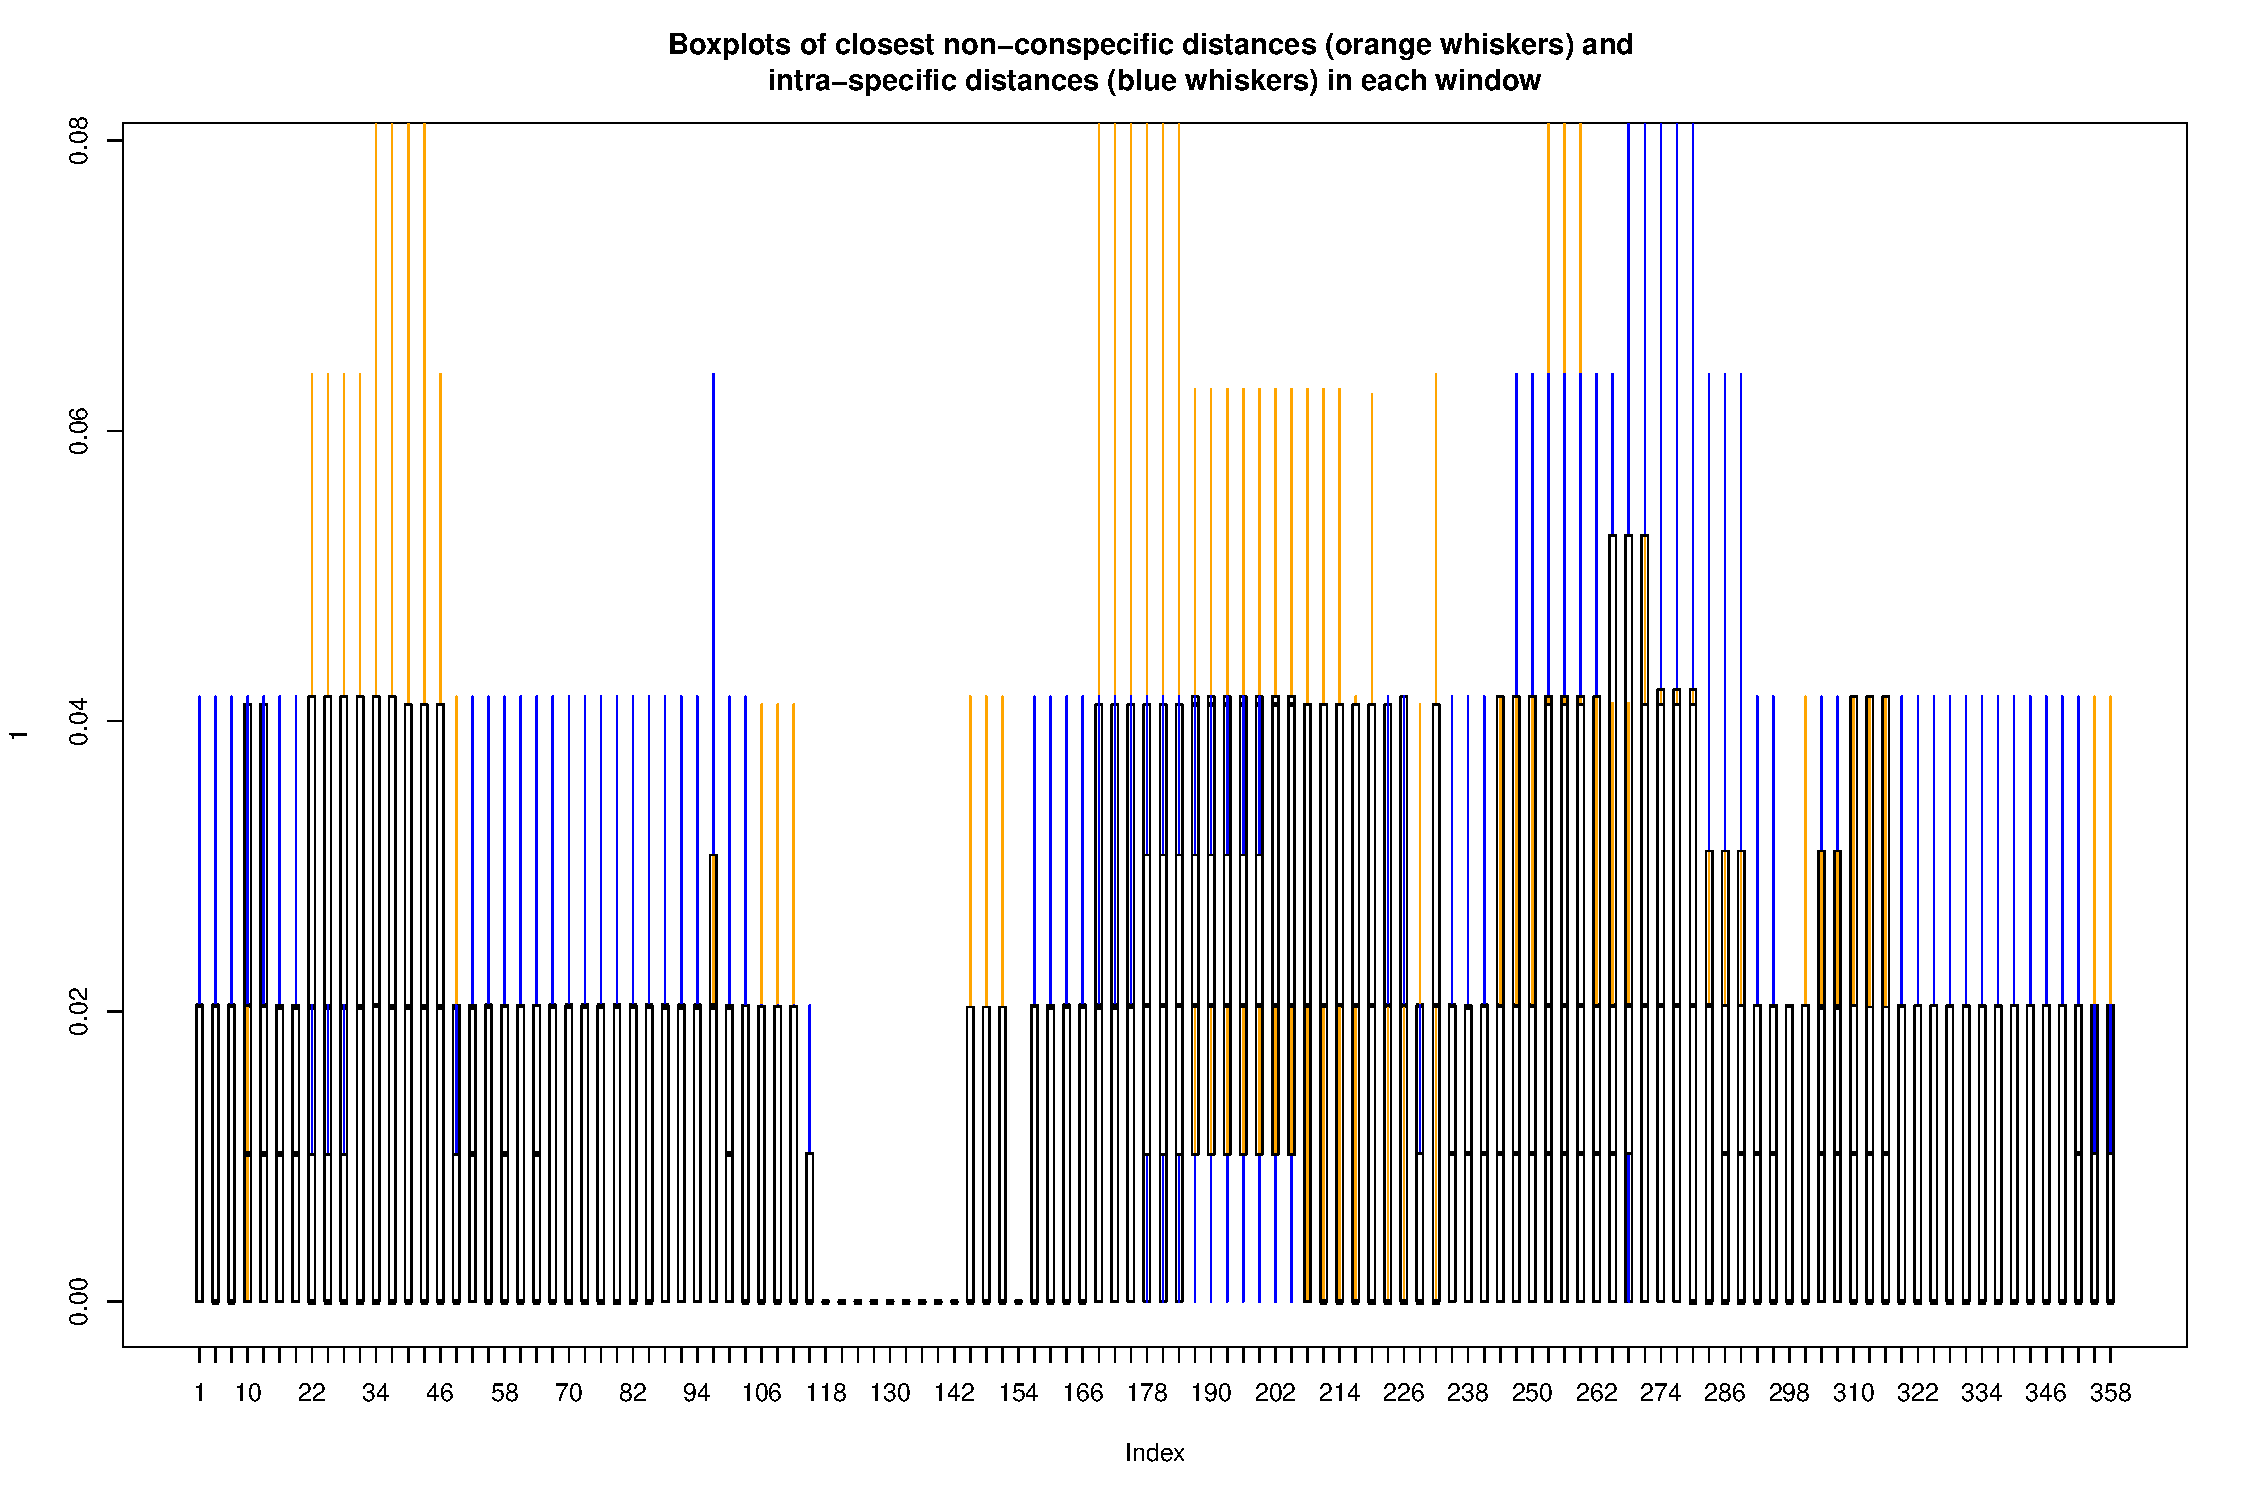
\includegraphics[width=0.9\textwidth]{slideBoxplots}
	\caption{Boxplots showing the distribution of the nearest non-conspecific (orange) and intraspecific (blue) distances across the COI sequences of \emph{Anoteropsis} spp.}
	\label{slideBoxplots.fig}
\end{figure}


When plotted, this function produces the graphic shown in Figure \ref{slideBoxplots.fig}. Unfortunately, there is very little difference between the intra and inter-specific distances at the 50 bp window size. Even the windows around the 200 bp position display significant overlap between the two measures, showing that there is no ``barcoding gap'' with this size of DNA fragment.

To look at a more conventional example of the barcoding gap we can have a look at the \fun{weevils} dataset (Figure \ref{weevilsBox.fig}):

\begin{console}
weevilsBox <- slideBoxplots(weevils, 50, weevilSpp1, interval="codons", 
method="nonCon")
plot(weevilsBox)
\end{console}

\begin{figure}[p]
	\centering
	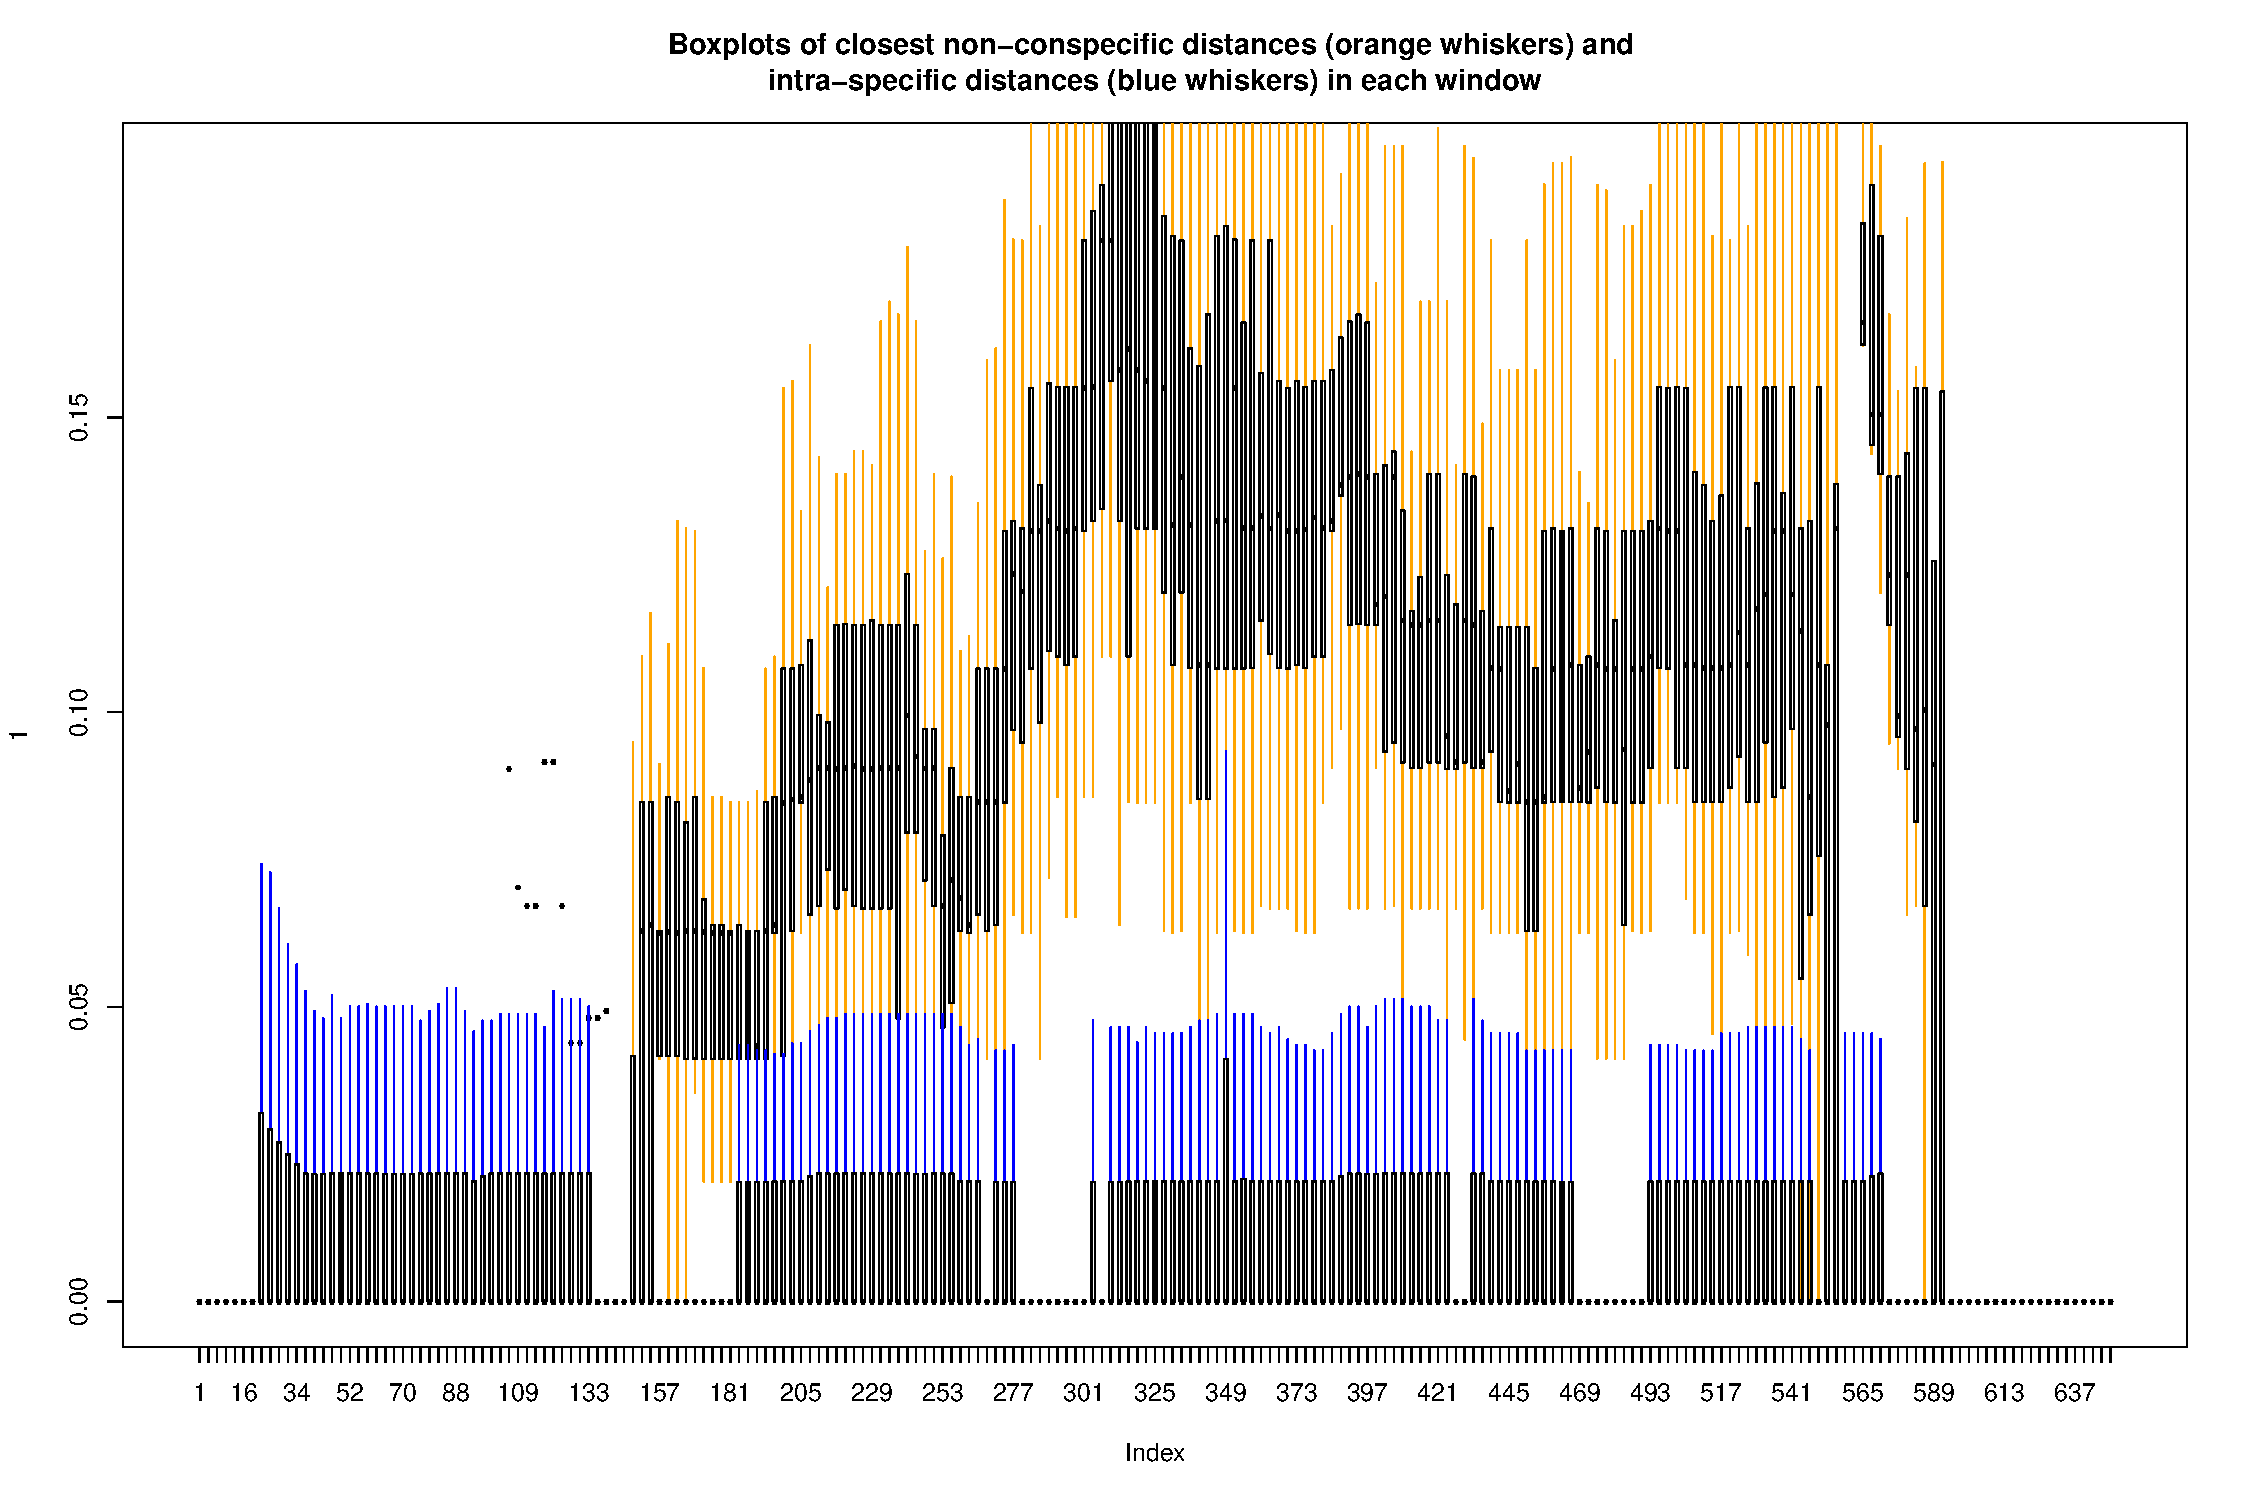
\includegraphics[width=0.9\textwidth]{weevilsBox}
	\caption{Boxplots showing the distribution of the nearest non-conspecific (orange) and intraspecific (blue) distances across the COI sequences of \emph{Trigonopterus} spp.\ weevils}
	\label{weevilsBox.fig}
\end{figure}

%####################################
%####################################
%####################################

\section{Conclusion}
This tutorial gives an introduction the the usage of some of the functions implemented in \spider, particularly with regards to its sliding window capabilities and use in DNA barcoding research. 
\Spider~is an actively developing package, and it is intended that further analyses will be developed within it, with an especial focus on the analysis of conflict in phylogenetic data, checks of alignment quality, tools for studying ancient DNA and further analyses for morphological and categorical data.
As the package matures, it is hoped that \spider~will be a valuable addition to toolkit of \progname{R} packages available for use in the field of taxonomy, systematics and molecular biology. For more information, or to get involved in the development of the package, please visit our site on R-Forge, \href{http://spider.r-forge.r-project.org/}{http://spider.r-forge.r-project.org/}.



\bibliography{tutorial_references}

\end{document}